\pdfminorversion=7
\documentclass[12pt]{article}
\usepackage[letterpaper,margin=1in]{geometry}
\usepackage[T1]{fontenc}
\usepackage[utf8]{inputenc}

\usepackage{amsmath,amssymb}
\usepackage{graphicx}
\usepackage{booktabs,longtable,array}
\usepackage[protrusion=true,expansion=false]{microtype}
\usepackage{caption}
\usepackage[hidelinks]{hyperref}
\setlength{\parindent}{0pt}
\setlength{\parskip}{0.65em}
\setlength{\LTpre}{0.5em}
\setlength{\LTpost}{0.5em}
\captionsetup{font=small,labelfont=bf}
\renewcommand{\arraystretch}{1.15}
\ifdefined\pdfinfoomitdate\pdfinfoomitdate=1\fi
\ifdefined\pdftrailerid\pdftrailerid{}\fi
\ifdefined\pdfsuppressptexinfo\pdfsuppressptexinfo=-1\fi
\hypersetup{pdftitle={From latent bandgap to measured edge in HgCdTe: distributional observation operators and structural identifiability},pdfauthor={Terence Fisher}}
\title{From latent bandgap to measured edge in HgCdTe: distributional observation operators and structural identifiability}
\author{Terence Fisher\\\small Brooks Photonics, Florida, USA}
\date{}
\begin{document}
\maketitle


\begin{abstract}

The bandgap of Hg1-xCdxTe is commonly treated as a scalar function of alloy composition and temperature, while reported optical edges also depend on local material-state distributions, carrier filling, absorption physics, optical geometry, and the selected observation operator. We develop an HgCdTe-specific forward framework that keeps these layers explicit and apply established structural-identifiability methods to determine which parameter combinations can be recovered from common band-edge measurements. Near the normal-to-inverted transition, existing latent-gap laws span 25.08 K in central critical temperature at mean composition x=0.155 before specimen-distribution uncertainty is introduced. A Gaussian distribution of local gaps reproduces the Herrmann approximately-s/2 apparent tail scale under source-aligned conditions, but changing only the fitted absorption window changes the inferred tail energy by 60.1\%. Combining the Chang exponential tail with a single-pass response gives the established logarithmic thickness shift, while an application-specific analysis shows that any number of tail-only cutoff measurements has Jacobian rank at most two for four nominal absorption parameters. A high-density synthetic sensitivity calculation shows that a parabolic Burstein-Moss treatment can overestimate a declared nonparabolic shift by 147 meV. A separate reproduction of Dingrong Table 1 exposes an 11.297 meV root-mean-square inconsistency between the printed finite-temperature density equation, the printed momentum matrix, and the reported Fermi elevations; the rounded rows imply a tightly clustered diagnostic momentum matrix near 8.51e-8 eV cm but do not establish a revised material constant. Finally, for the declared Gaussian-gap, power-law, uniform-carrier-translation, single-pass model, the five nominal parameters (latent gap, carrier translation, gap width, absorption amplitude, effective thickness) enter only through the translated mean gap, gap width, and amplitude-thickness product. The corresponding dense-spectrum Jacobian has rank at most three. A controlled nontranslational carrier marker raises rank to four but leaves one combined scaling-translation invariance. The contribution is an HgCdTe optical-metrology and inverse-problem synthesis: source-grounded forward operators, explicit identifiable combinations, quantitative observation-operator effects, and measurement requirements for latent-gap recovery.

\end{abstract}
\section{Introduction}

Hg1-xCdxTe occupies an unusually demanding metrological regime. Its signed zone-center gap can be tuned through zero by composition and temperature, its bands are strongly nonparabolic, and its optical edge is sensitive to carrier state, disorder, processing, thickness, and the analysis operator. Quantities reported as ``the bandgap'' may therefore refer to absorption, photoconductivity, photoluminescence, magneto-optical transitions, or detector cutoff and need not represent the same latent material coordinate.

Engineering equations such as the Hansen relation remain useful as latent mean-gap baselines. Their numerical precision should not be confused with the precision of an experimental observation. The previous study in this repository showed that historical composition uncertainty, source lineage, carrier and vacancy state, and edge-definition choice dominate the sub-meV ordering of common empirical laws. The historical evidence did not identify a universal replacement equation.

The present work develops a constructive counterpart. Rather than selecting another scalar gap equation, it asks:

\begin{quote}\itshape
Given a latent signed band structure, a specimen-state distribution, a carrier state, an optical geometry, and a measurement operator, what observable edge will the experiment report?
\end{quote}

Structural identifiability, output-preserving parameter symmetries, and identifiable parameter combinations are established ideas in inverse-problem theory. \cite{bellman_astrom_1970,yates_evans_chappell_2009,eisenberg_hayashi_2014} Beer-Lambert attenuation likewise contains the familiar product of absorption strength and optical path length. We do not claim these general principles as new. We apply them to a source-grounded HgCdTe forward hierarchy and derive the explicit parameter combinations, rank bounds, counterexamples, and measurement-design consequences of the declared model.

The principal contributions are:

\begin{enumerate}
\item bounded-Gaussian propagation from composition variation to local-gap and critical-temperature distributions, including no-crossing censoring;
\item an independent reproduction of the Herrmann Gaussian-gap-to-apparent-tail scale and a quantified 60.1\% fit-window non-uniqueness result;
\item a source-bounded Chang absorption-to-detector-cutoff operator and a model-specific rank-two bound for tail-only cutoff datasets;
\item a nonparabolic carrier-filling sensitivity analysis, plus a finite-temperature reproduction and source-consistency audit of Dingrong Table 1;
\item an application-specific rank-three bound for the declared distributed single-state spectrum and a machine-precision counterexample;
\item a measurement-design prescription identifying the independent information required for latent-gap recovery.
\end{enumerate}

The paper is framed as semiconductor optical metrology and inverse-problem methods for HgCdTe. It is not a new general theory of structural identifiability, a universal HgCdTe bandgap equation, or a complete microscopic absorption model.

\section{Forward hierarchy}
\begin{figure}[p]
\centering
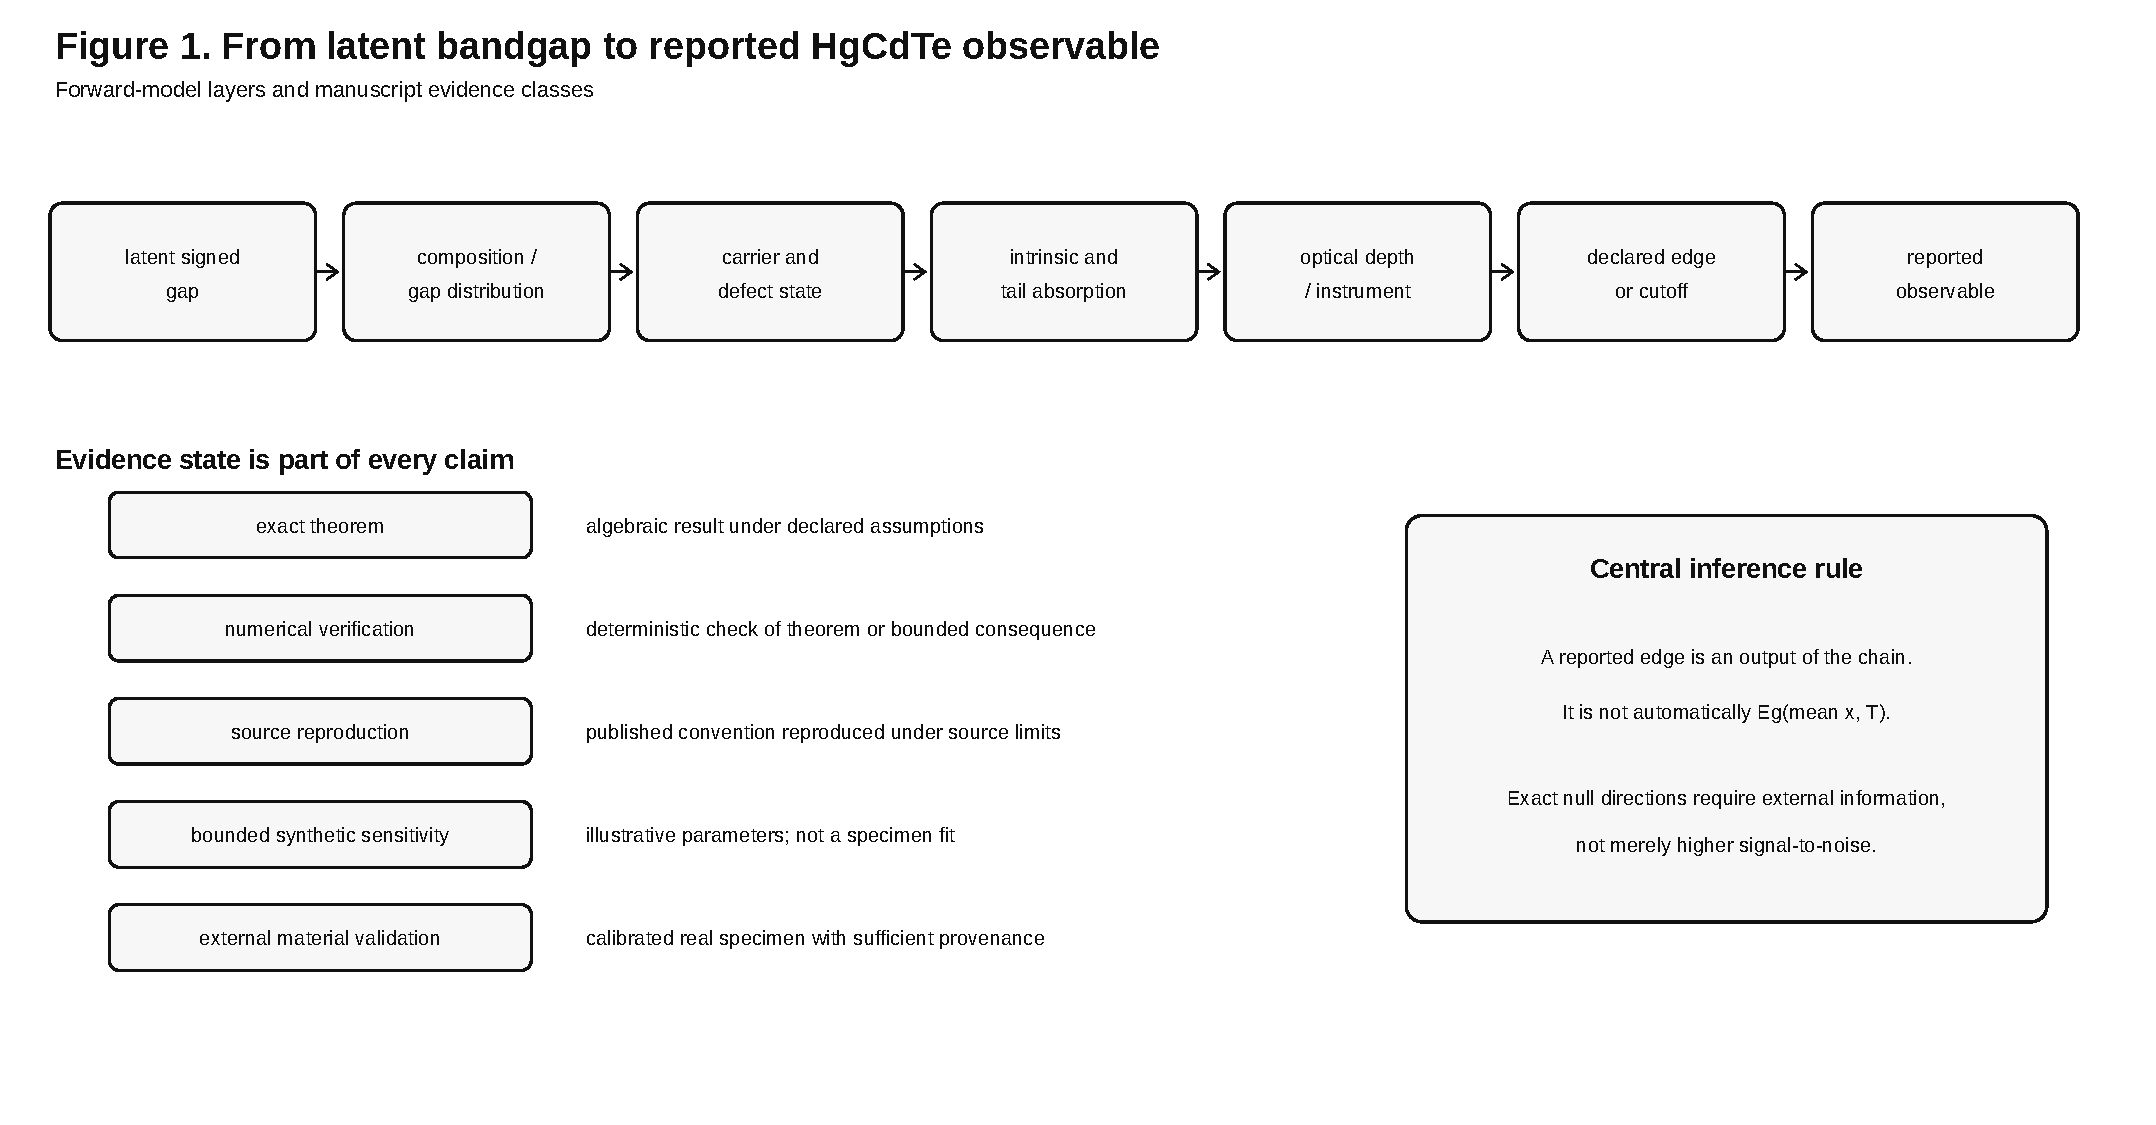
\includegraphics[width=\textwidth,height=0.82\textheight,keepaspectratio]{figures/figure1_forward_hierarchy.pdf}
\caption{Forward hierarchy from latent signed gap to reported observable and the evidence classes used throughout the study.}
\label{fig:figure1:forward:hierarchy}
\end{figure}
\clearpage

The controlling forward sequence is

\begin{verbatim}
latent signed gap
-> composition and local-gap distribution
-> carrier and defect state
-> intrinsic, tail, and free-carrier absorption
-> effective optical thickness and instrument response
-> declared edge or cutoff operator
-> reported observable
\end{verbatim}

Each stage introduces parameters that may be observable only through combinations with parameters from another stage.

\subsection{Latent signed gap}

Let

\[
E_g^{(0)}(x,T)=E_{\Gamma_6}(x,T)-E_{\Gamma_8}(x,T)
\]

be the latent signed zone-center gap of a declared mean material state. The superscript \texttt{(0)} distinguishes this latent reference from an observed optical edge. The framework does not select one universal equation for $E_g^{(0)}$; Hansen, reconstructed Laurenti, and archived constrained candidates are retained as alternative latent laws when model dependence must be quantified.

\subsection{Composition and local-gap distributions}

Let

\[
X=\bar x+\delta x,
\qquad
\mathbb E[\delta x]=0,
\qquad
\operatorname{Var}(X)=\sigma_x^2.
\]

For sufficiently narrow composition variation,

\[
\mathbb E[E_g(X,T)]
\approx
E_g(\bar x,T)+\frac12E_{g,xx}(\bar x,T)\sigma_x^2,
\]

and

\[
\sigma_{E,x}\approx |E_{g,x}(\bar x,T)|\sigma_x.
\]

Near a simple zero-gap root,

\[
\sigma_{T_c}
\approx
\left|\frac{E_{g,x}}{E_{g,T}}\right|\sigma_x.
\]

Exact deterministic quadrature over a Gaussian composition model conditioned on $0\le x\le1$ is used when local propagation fails, when roots are absent, or when conditional-root distributions become censored.

\subsection{Distributed absorption}

For a local gap $G$, use the controlled local-edge family

\[
\alpha_{\mathrm{loc}}(E\mid G)=A(E-G)_+^p,
\]

where $(y)_+=\max(y,0)$ and $p$ is declared. For

\[
G\sim\mathcal N(\mu_G,\sigma_G^2),
\]

the convolved absorption has the scale form

\[
\bar\alpha(E)
=A\sigma_G^p
F_p\left(\frac{E-\mu_G}{\sigma_G}\right),
\]

with

\[
F_p(z)=\int_{-\infty}^{z}(z-u)^p\phi(u)\,du.
\]

This is a controlled observation basis, not a complete microscopic HgCdTe absorption law.

\subsection{Detector response and operational cutoff}

For effective absorbing thickness $d$, the reduced single-pass response is

\[
R(E,d)=1-\exp[-\alpha(E)d].
\]

A target response $R_t$ corresponds to

\[
\alpha_t=-\frac{\ln(1-R_t)}{d}.
\]

If the crossing lies on an exponential tail joined at $(E_j,\alpha_j)$,

\[
\alpha(E)=\alpha_j\exp\left(\frac{E-E_j}{W}\right),
\]

then

\[
E_c=E_j+W\ln\left(\frac{\alpha_t}{\alpha_j}\right).
\]

The reduced operator inherits the standard optical-depth product dependence. \cite{iupac_beer_lambert_2025} Effective thickness is an observation-model quantity and is not assumed equal to physical film thickness.

\subsection{Carrier-filled optical edge}

A declared zero-temperature spherical sensitivity model uses

\[
k_F=\left(\frac{3\pi^2n}{g_v}\right)^{1/3},
\qquad
E_{\mathrm{par}}=\frac{\hbar^2k_F^2}{2m_e^*},
\]

and the Kane-type dispersion

\[
E_c(1+\alpha E_c)=E_{\mathrm{par}},
\]

with positive solution

\[
E_c=
\frac{2E_{\mathrm{par}}}
{1+\sqrt{1+4\alpha E_{\mathrm{par}}}}.
\]

The observed edge is kept decomposed:

\[
E_{\mathrm{opt}}
=E_g^{(0)}
+\Delta E_{\mathrm{BM}}
+\Delta E_{\mathrm{BGR}}
+\Delta E_{\mathrm{obs}}.
\]

Burstein-Moss filling is not conflated with band-gap renormalization.

For the real Dingrong specimen, the source's finite-temperature carrier-density integral is implemented separately rather than replacing it with the zero-temperature sensitivity model.

\section{Methods and evidence classes}

\subsection{Evidence classes}

Every result is assigned one of five evidence states:

\begin{enumerate}
\item exact analytical statement under declared assumptions;
\item deterministic numerical verification;
\item source-conditioned reproduction;
\item bounded synthetic sensitivity;
\item external material validation.
\end{enumerate}

Only the fifth state supports unrestricted specimen-level claims. Theorem labels identify exact statements under their assumptions; they do not imply unprecedented mathematics.

\subsection{Numerical quadrature}

Gaussian gap convolutions are evaluated with energy-dependent Gauss-Legendre quadrature restricted to $G\le E$. Splitting the integral at the moving threshold removes an interior cusp and yields stable convergence. Linear and quadratic edge branches are checked against closed Gaussian moments.

Bounded composition distributions use deterministic Gaussian quadrature conditioned on the physical alloy interval. Transition roots are classified as single crossing, always normal, always inverted, multiple crossing, or unresolved before conditional moments are reported.

Dingrong's finite-temperature density equation is solved by deterministic quadrature and scalar inversion at each of the four reported temperatures.

\subsection{Structural identifiability}

For observables $y(\theta)$, local sensitivity is represented by

\[
J_{ij}=\frac{\partial y_i}{\partial\theta_j}.
\]

Exact output-preserving transformations and identifiable combinations are derived before numerical singular values are interpreted. Numerical rank verifies the analytical result but does not define it when an exact invariance is available.

\subsection{Prior-art boundary}

The general concepts of structural identifiability, parameter symmetry, and identifiable parameter combinations are established. The amplitude-thickness product is inherited from Beer-Lambert optical depth. Thin-film optical inversion literature likewise shows that thickness and optical constants require sufficiently informative combinations of transmission, reflection, interference, angle, polarization, or external constraints. \cite{chambouleyron_1997,babeva_kitova_konstantinov_2001_error,babeva_kitova_konstantinov_2001_unique,mendoza_galvan_2021}

HgCdTe-specific source boundaries are:

\begin{itemize}
\item Herrmann et al. establish that a Gaussian-like gap distribution can generate a near-exponential tail and report the approximately-$s/2$ scale; \cite{herrmann_1992}
\item Chang et al. establish the nonparabolic intrinsic plus Urbach absorption model and the importance of effective absorber thickness for detector cutoff; \cite{chang_2006,chang_2007}
\item Dingrong et al. establish finite-temperature carrier filling and below-gap free-carrier absorption in a real degenerate specimen; \cite{dingrong_1985}
\item Teppe et al. establish a temperature-driven near-critical Kane-mass series. \cite{teppe_2016}
\end{itemize}

The candidate contribution is the HgCdTe-specific synthesis, explicit parameter combinations, model-specific rank bounds, exact counterexamples, and quantitative measurement consequences.

\section{Results}

\subsection{Composition distributions broaden and censor the apparent transition}
\begin{figure}[p]
\centering
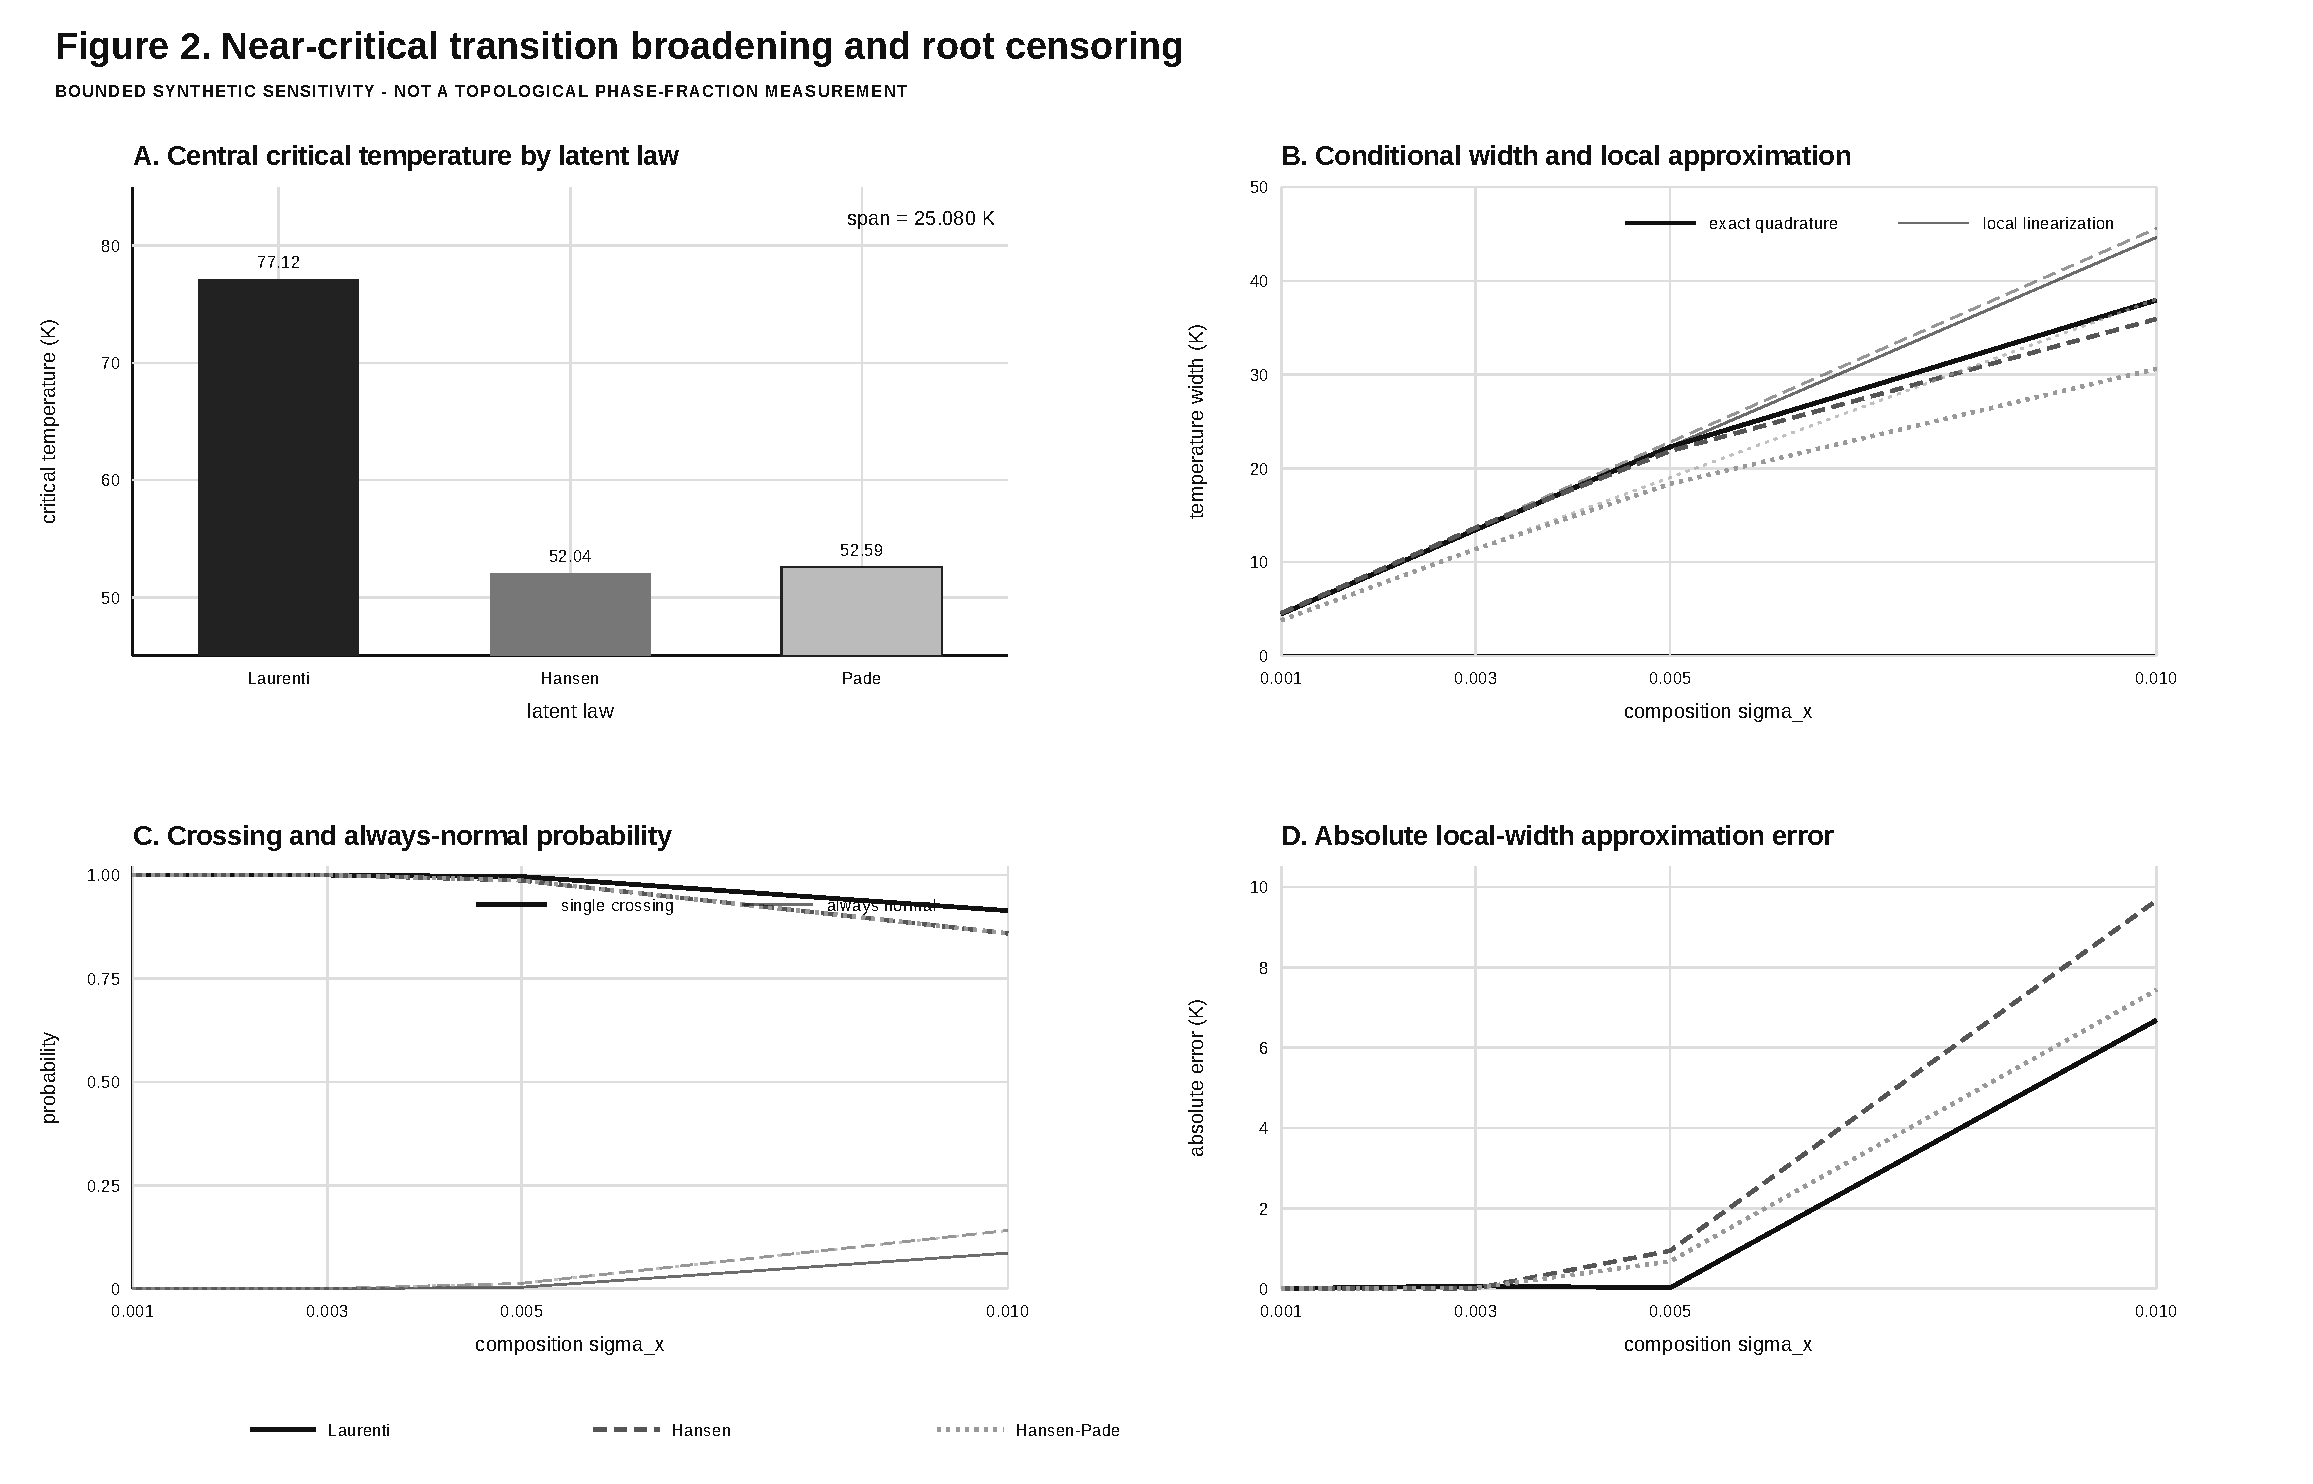
\includegraphics[width=\textwidth,height=0.82\textheight,keepaspectratio]{figures/figure2_transition_distribution.pdf}
\caption{Model-conditioned near-critical transition distributions, crossing probabilities, and local-approximation error.}
\label{fig:figure2:transition:distribution}
\end{figure}
\clearpage

At nominal mean composition $\bar x=0.155$, the retained latent laws predict:

\begingroup
\scriptsize
\begin{longtable}{@{}p{0.350\linewidth}p{0.590\linewidth}@{}}
\toprule
\textbf{Latent law} & \textbf{Central $T_c$} \\
\midrule
\endfirsthead
\toprule
\textbf{Latent law} & \textbf{Central $T_c$} \\
\midrule
\endhead
Reconstructed Laurenti & 77.1241 K \\
Hansen-Schmit-Casselman & 52.0438 K \\
Archived Hansen-Pade & 52.5937 K \\
\bottomrule
\end{longtable}
\endgroup

The central span is

\[
25.0803\ \mathrm K.
\]

At $\sigma_x=0.001$, exact composition-induced widths are \texttt{3.804-4.560 K}, so latent-law choice dominates. At $\sigma_x=0.005$, conditional widths become \texttt{18.345-22.290 K}, while \texttt{0.36-1.30\%} of the declared distribution remains normal throughout \texttt{0-300 K}. At $\sigma_x=0.010$, the always-normal fraction rises to \texttt{8.60-14.12\%}.

No-crossing compositions are excluded from the conditional root distribution. At $\sigma_x=0.010$, conditional means shift by \texttt{5.52-11.05 K}, while local linear propagation overstates conditional width by \texttt{6.68-9.66 K}.

These are model-conditioned transition statistics, not measured topological phase fractions.

\subsection{A Gaussian gap distribution produces an apparent tail but not a unique inverse width}
\begin{figure}[p]
\centering
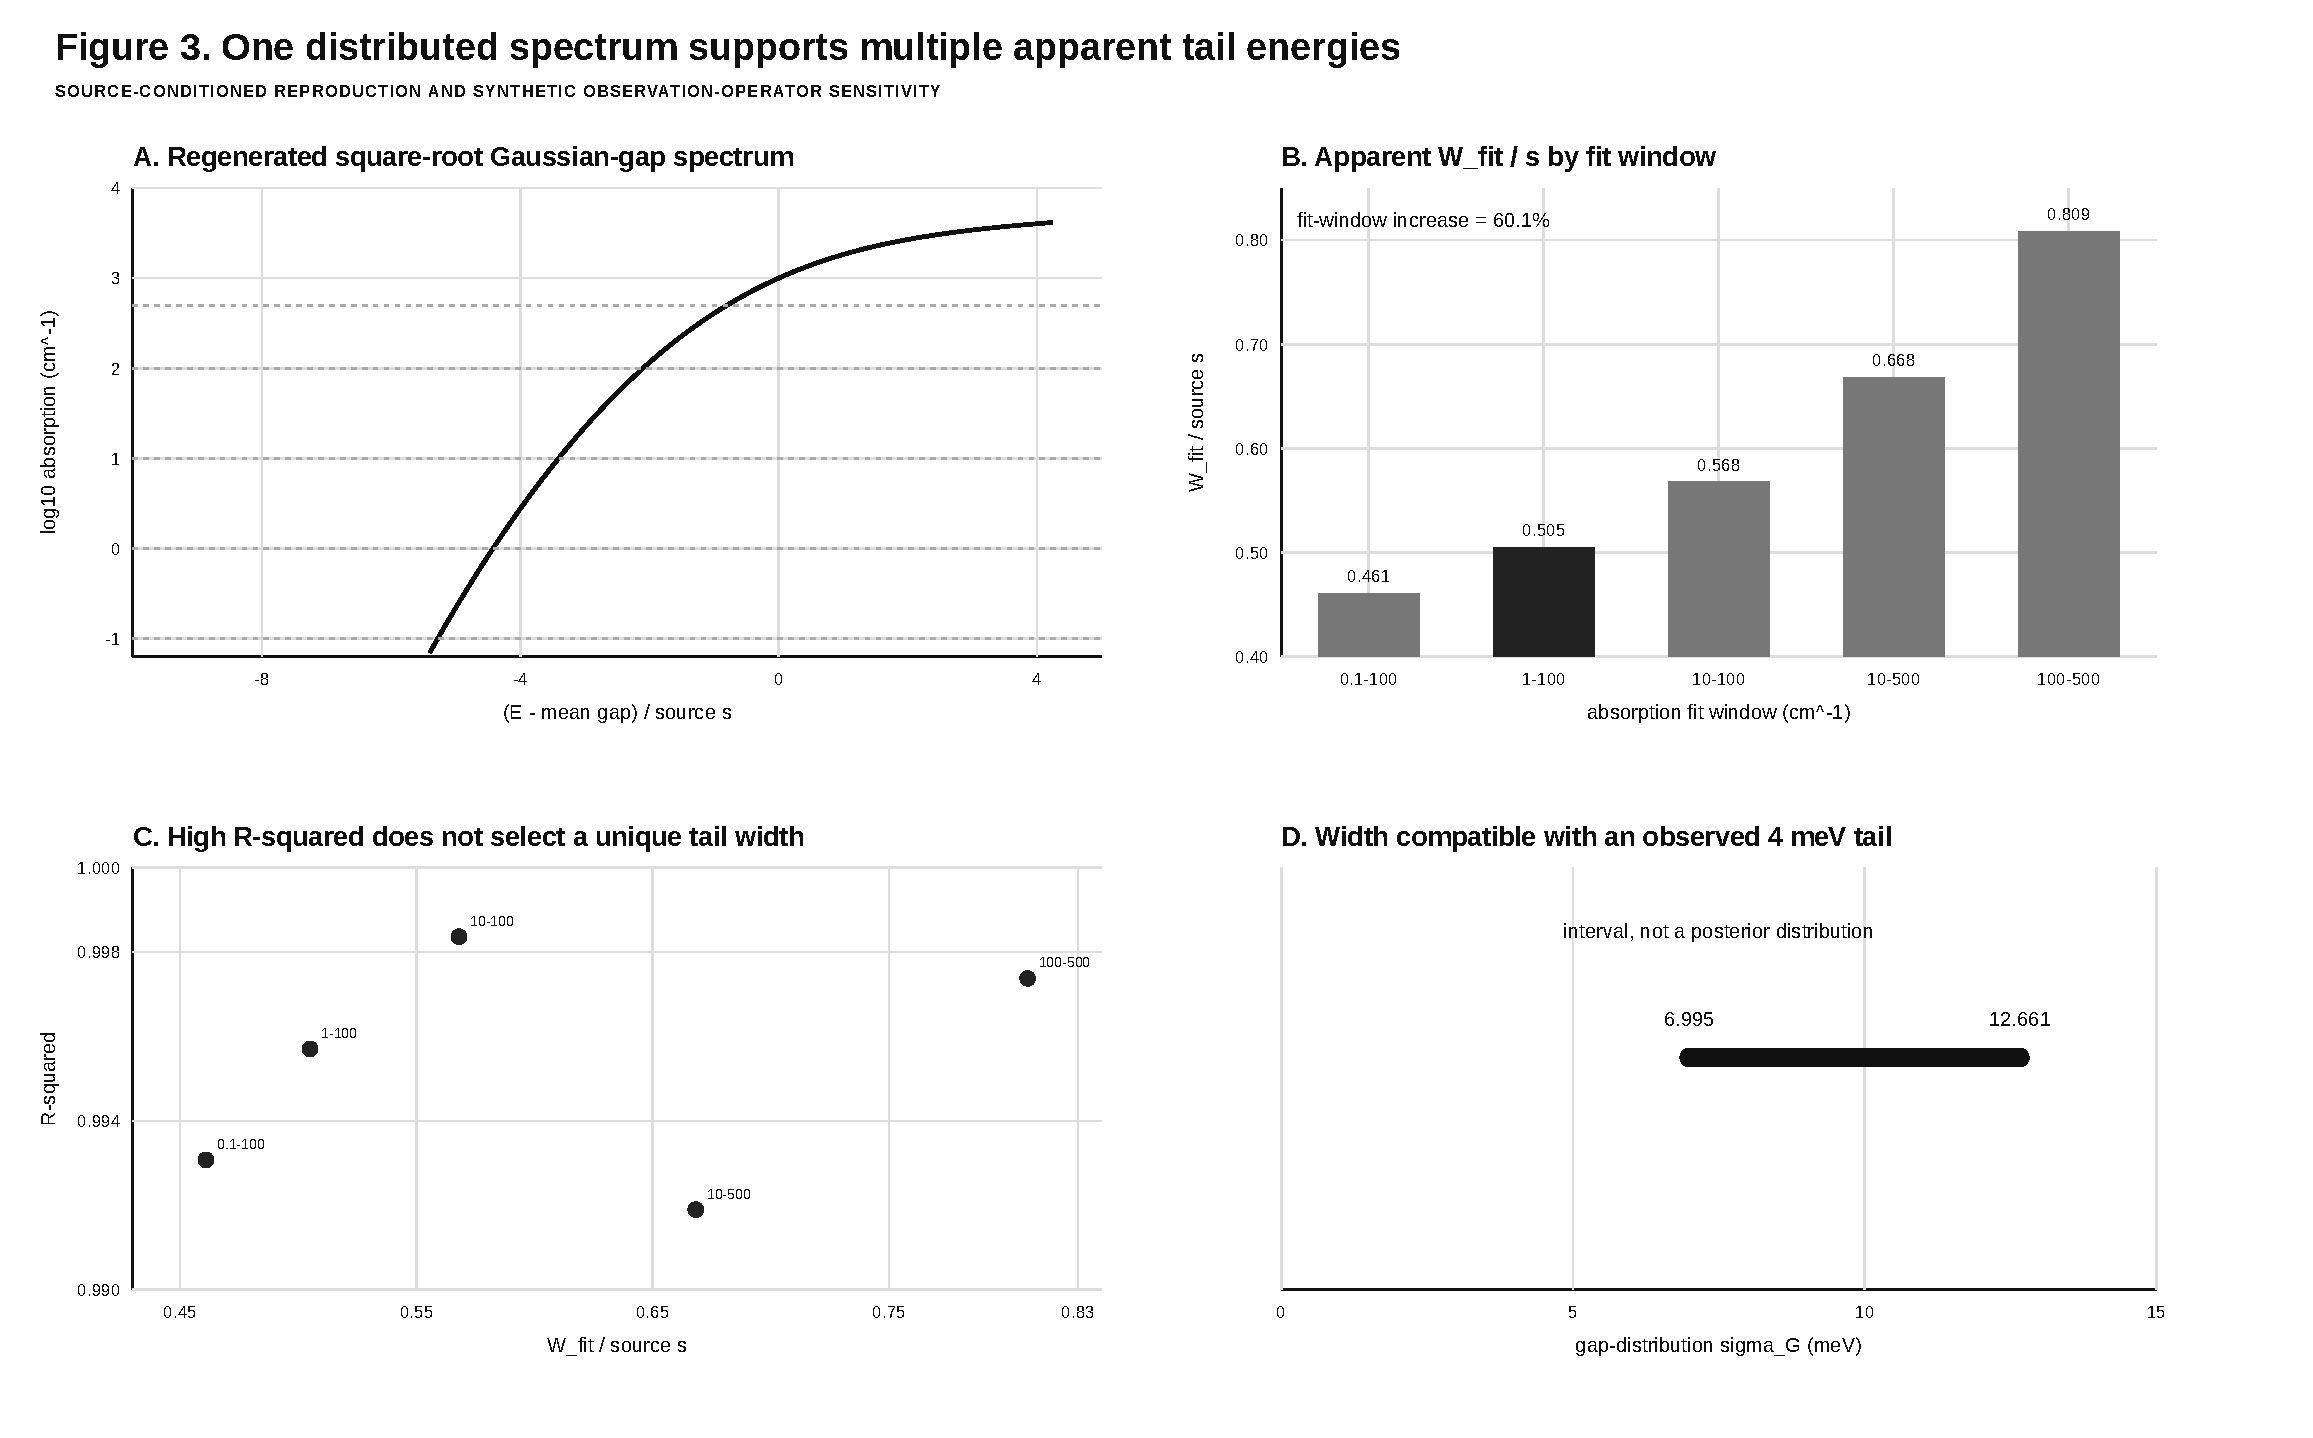
\includegraphics[width=\textwidth,height=0.82\textheight,keepaspectratio]{figures/figure3_herrmann_tail_nonuniqueness.pdf}
\caption{Source-conditioned Gaussian-gap convolution and fit-window dependence of the apparent exponential-tail energy.}
\label{fig:figure3:herrmann:tail:nonuniqueness}
\end{figure}
\clearpage

Herrmann et al. use

\[
P(G)=\frac{1}{2s\sqrt\pi}
\exp\left[-\frac{(G-\bar G)^2}{4s^2}\right],
\]

so

\[
\sigma_G=\sqrt2\,s.
\]

For a square-root local edge and the source-stated \texttt{1-100 cm\textasciicircum{}-1} interval, the reproduction gives

\[
W_{\mathrm{fit}}/s=0.50504,
\qquad
R^2=0.99570.
\]

The same spectrum is not exactly exponential:

\begingroup
\scriptsize
\begin{longtable}{@{}p{0.220\linewidth}p{0.280\linewidth}p{0.440\linewidth}@{}}
\toprule
\textbf{Fit window ($\mathrm{cm^{-1}}$)} & \textbf{$W_{\mathrm{fit}}/s$} & \textbf{$R^2$} \\
\midrule
\endfirsthead
\toprule
\textbf{Fit window ($\mathrm{cm^{-1}}$)} & \textbf{$W_{\mathrm{fit}}/s$} & \textbf{$R^2$} \\
\midrule
\endhead
0.1-100 & 0.46096 & 0.99307 \\
1-100 & 0.50504 & 0.99570 \\
10-100 & 0.56806 & 0.99836 \\
10-500 & 0.66828 & 0.99190 \\
100-500 & 0.80871 & 0.99738 \\
\bottomrule
\end{longtable}
\endgroup

Changing only the fit window from \texttt{1-100} to \texttt{100-500 cm\textasciicircum{}-1} increases the fitted tail energy by \texttt{60.1\%}, despite strong log-linear fits in both windows. Across the declared exponent and window family, an observed $W_{\mathrm{fit}}=4$ meV permits

\[
6.995\ \mathrm{meV}
\le \sigma_G \le
12.661\ \mathrm{meV}.
\]

The source mechanism is prior art. The quantified observation-window non-uniqueness is the project-specific result.

\subsection{Tail-only cutoff data identify at most two combinations}
\begin{figure}[p]
\centering
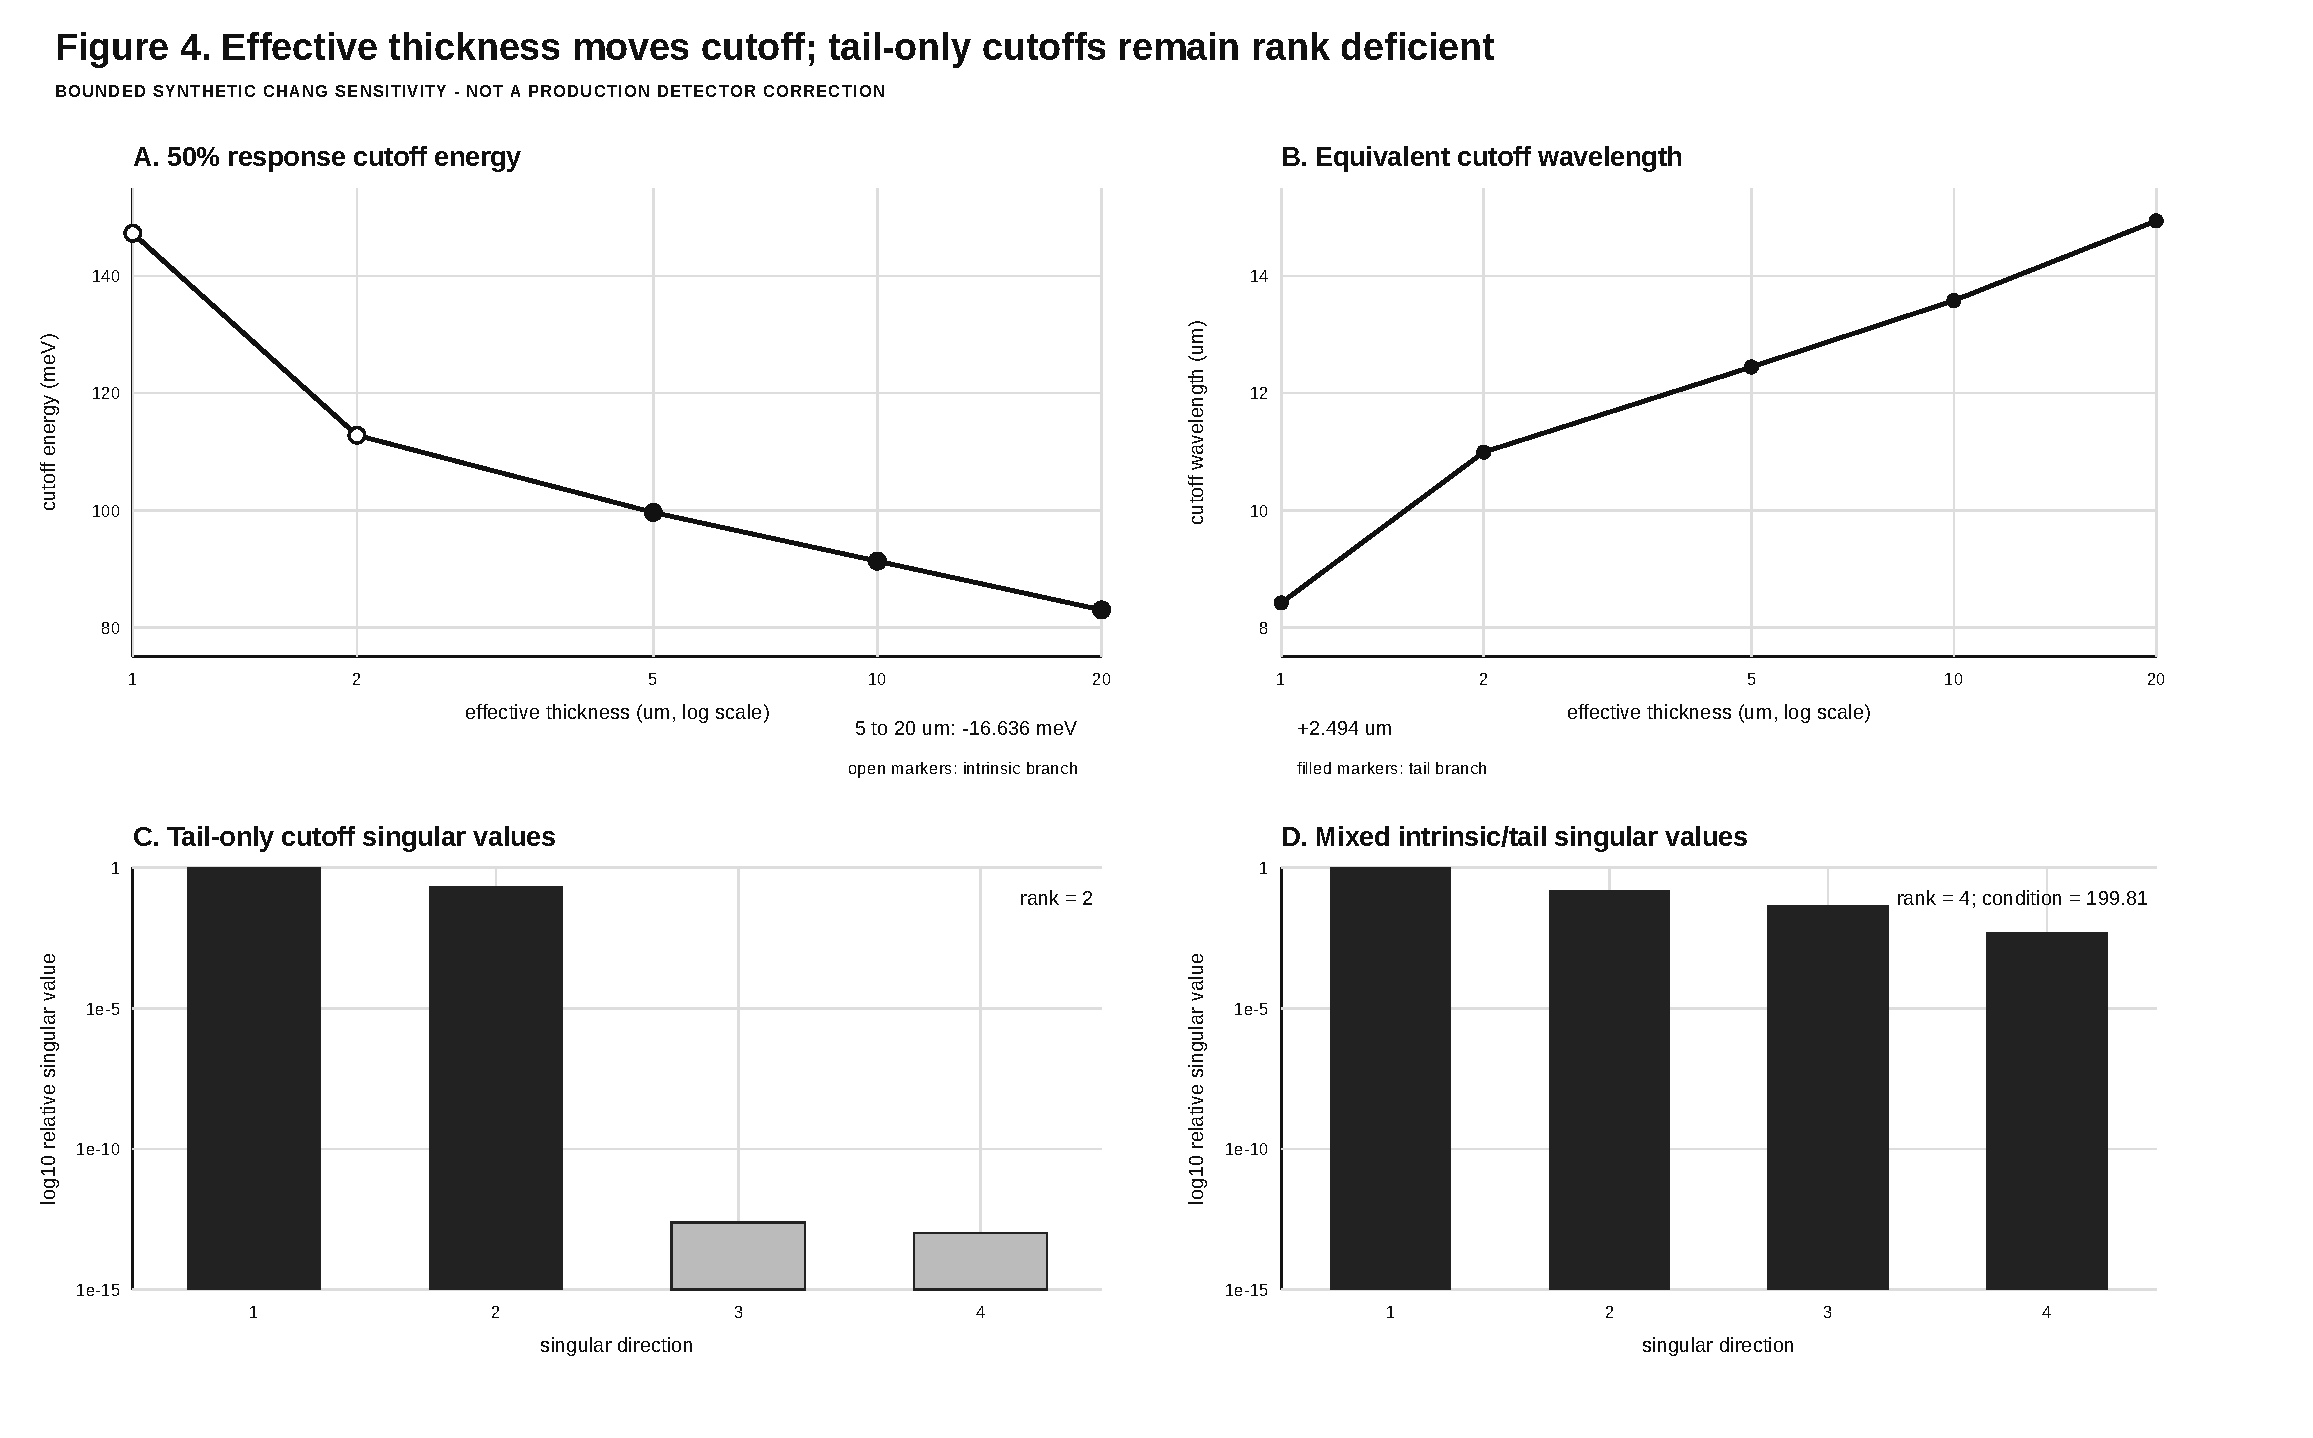
\includegraphics[width=\textwidth,height=0.82\textheight,keepaspectratio]{figures/figure4_chang_cutoff_rank.pdf}
\caption{Effective-thickness-dependent cutoff and structural-rank diagnostics for the source-bounded Chang operator.}
\label{fig:figure4:chang:cutoff:rank}
\end{figure}
\clearpage

Combining the Chang exponential tail with the single-pass target response gives

\[
E_c(d_2)-E_c(d_1)=-W\ln(d_2/d_1).
\]

The thickness dependence is established physics, not a new discovery. In the declared synthetic Chang case with $W=12$ meV, changing effective thickness from 5 to 20 $\mu$m moves the 50\% cutoff by

\[
-16.636\ \mathrm{meV},
\]

or from \texttt{12.445 um} to \texttt{14.939 um}, without changing the latent gap.

A tail-only cutoff can be written

\[
E_{c,i}=C(E_g,W,A,b)+WL_i,
\]

where $L_i$ depends only on effective thickness and response criterion. For

\[
\theta=(E_g,W,\ln A,\ln b),
\]

each Jacobian row has the form

\[
\nabla C+L_i\nabla W.
\]

Hence the row space has dimension at most two:

\[
\boxed{\operatorname{rank}(J_{\mathrm{tail}})\le2}.
\]

This is an application-specific analytical consequence of the affine cutoff family, not a new general theorem for every detector model. Nine tail-only observations give two finite singular values and two near-null directions. Mixed intrinsic and tail observations restore local rank four in the declared design, but the condition number remains \texttt{199.81}.

The Chang 2007 thickness curve is calculated and is not treated as independent external validation.

\subsection{Nonparabolic carrier filling can be a large correction}
\begin{figure}[p]
\centering
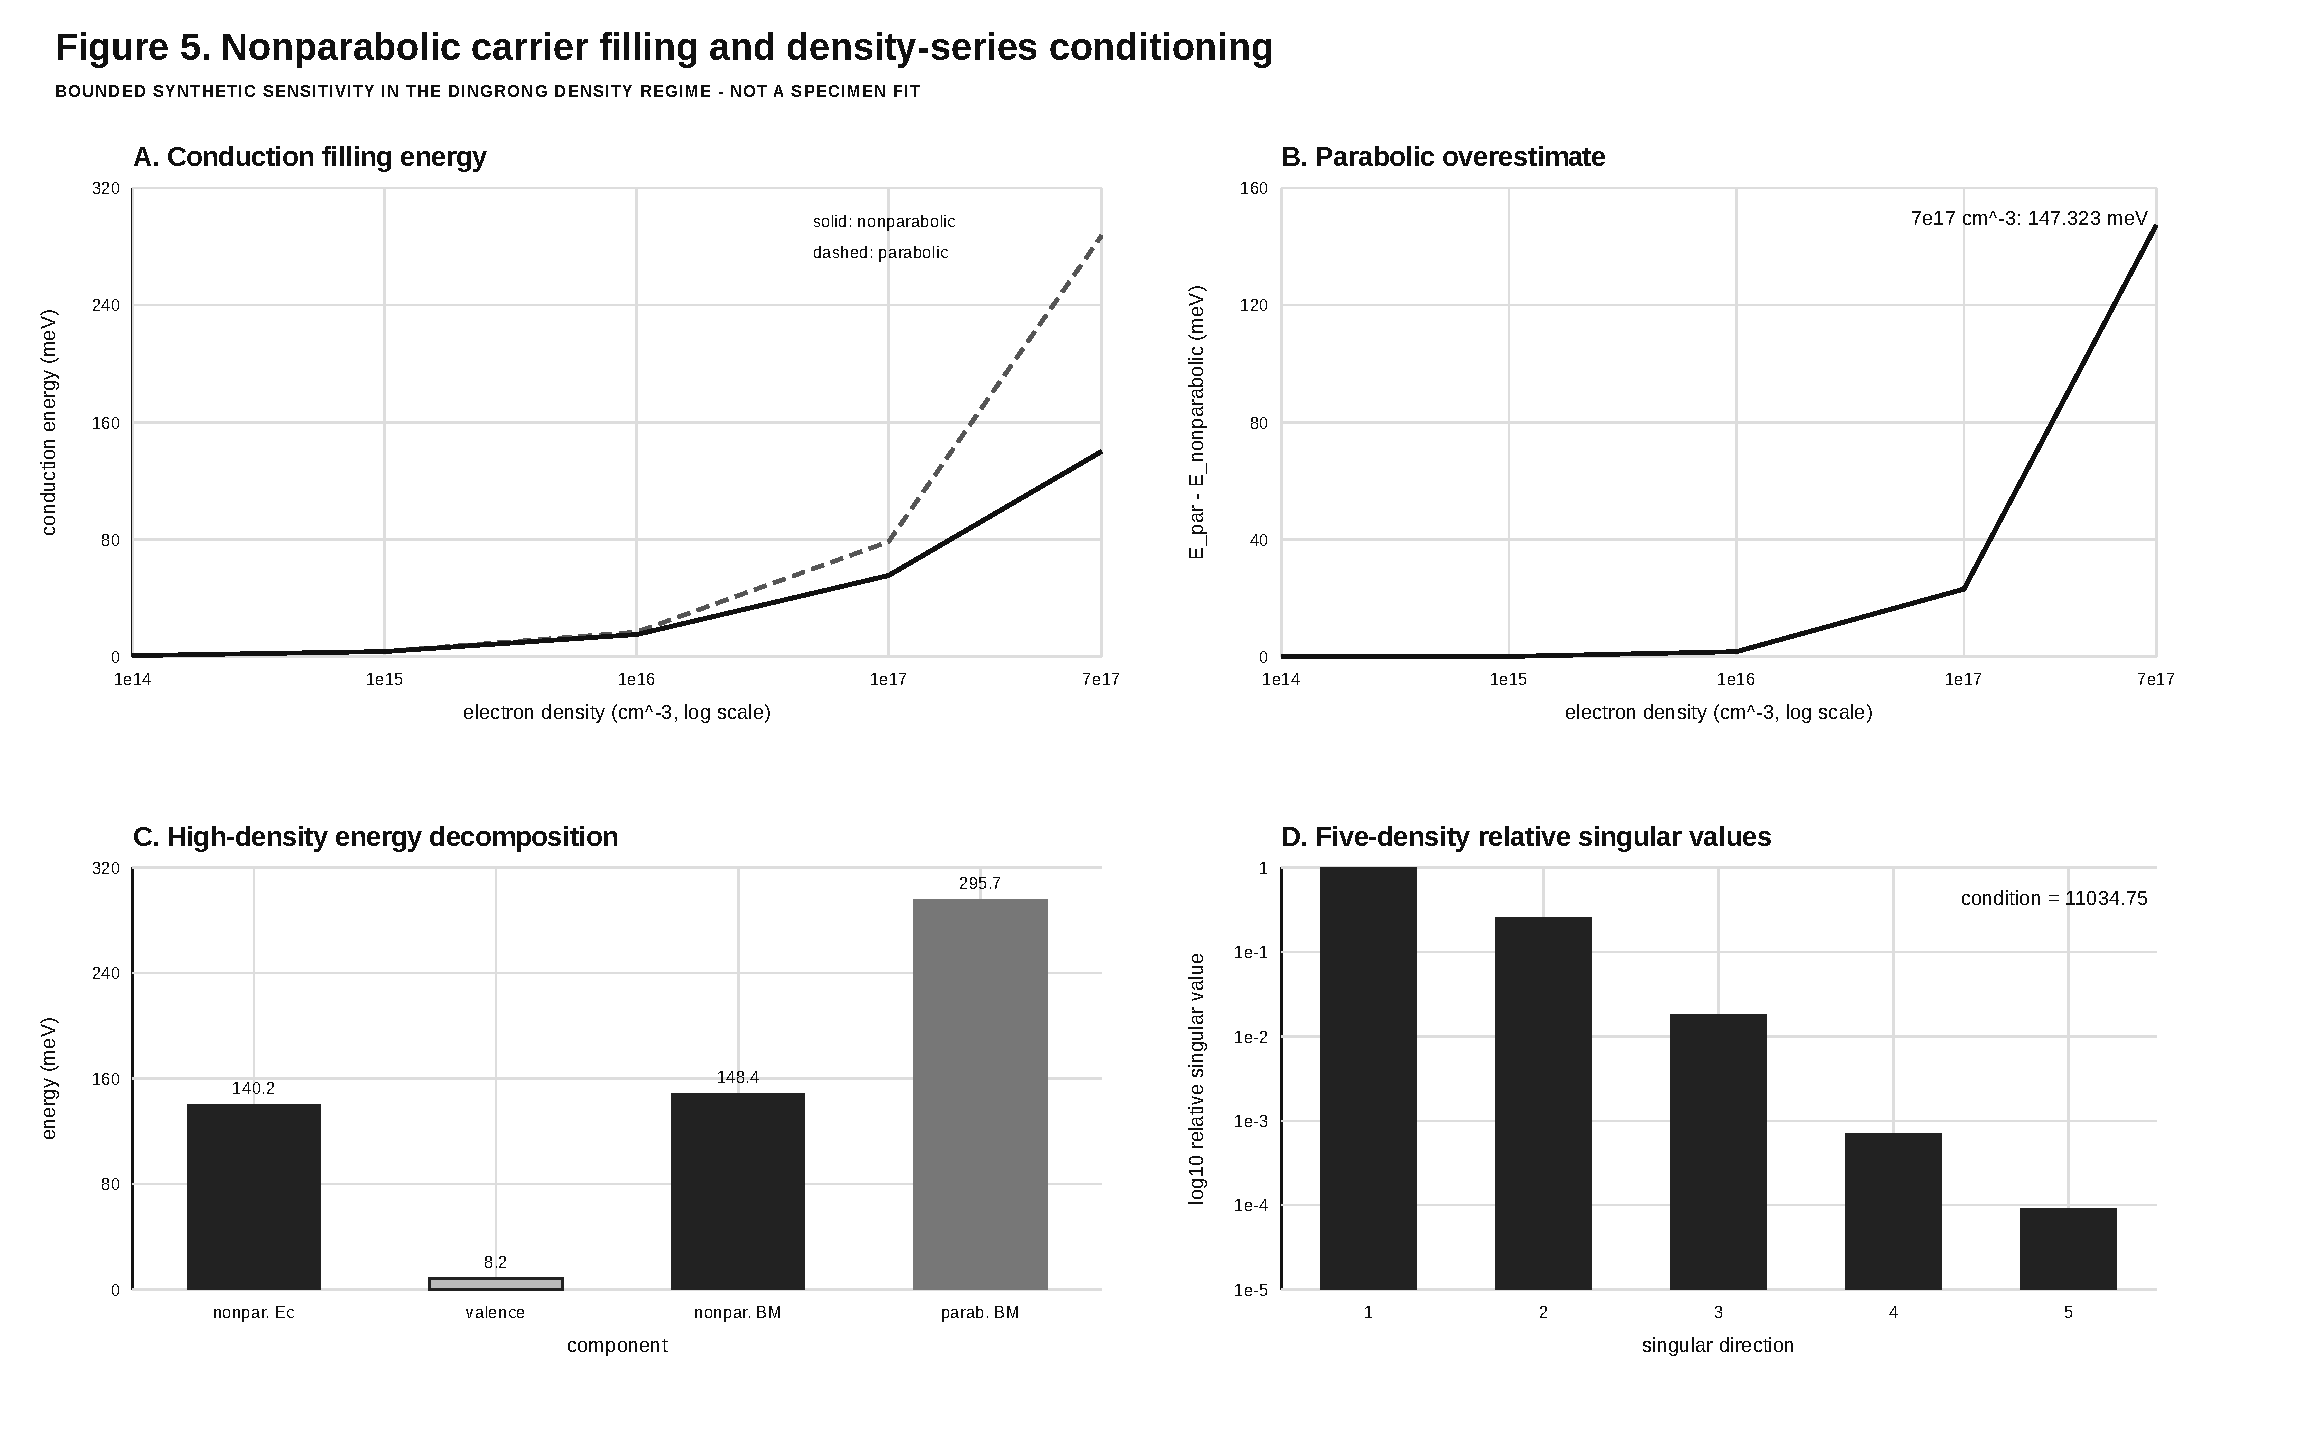
\includegraphics[width=\textwidth,height=0.82\textheight,keepaspectratio]{figures/figure5_carrier_filling.pdf}
\caption{Parabolic and nonparabolic carrier-filling sensitivity and density-series conditioning for the declared illustrative parameters.}
\label{fig:figure5:carrier:filling}
\end{figure}
\clearpage

Let

\[
q=\alpha E_{\mathrm{par}}.
\]

The declared zero-temperature sensitivity model gives

\[
\frac{E_{\mathrm{par}}-E_c}{E_c}
=
\frac{\sqrt{1+4q}-1}{2}.
\]

For

\begin{verbatim}
n          = 7.0e17 cm^-3
m_edge     = 0.010 m0
alpha      = 7.5 eV^-1
m_valence  = 0.35 m0
\end{verbatim}

we obtain:

\begingroup
\scriptsize
\begin{longtable}{@{}p{0.350\linewidth}p{0.590\linewidth}@{}}
\toprule
\textbf{Quantity} & \textbf{Value} \\
\midrule
\endfirsthead
\toprule
\textbf{Quantity} & \textbf{Value} \\
\midrule
\endhead
$k_F$ & 0.0274688 $\mathrm{\mathring{A}^{-1}}$ \\
Parabolic conduction energy & 287.476 meV \\
Nonparabolic conduction energy & 140.154 meV \\
Valence recoil & 8.214 meV \\
Nonparabolic BM shift & 148.367 meV \\
Parabolic BM shift & 295.690 meV \\
Parabolic overestimate & 147.323 meV \\
\bottomrule
\end{longtable}
\endgroup

A five-density series is locally rank five for the declared parameters but has condition number

\[
1.1035\times10^4.
\]

Formal full rank does not imply a stable unconstrained inversion. This sensitivity case is not a fit to the Dingrong specimen.

\subsection{Dingrong Table 1 provides a qualified real-specimen source test}

Dingrong et al. report an In-doped specimen with

\begin{verbatim}
composition x             0.19
carrier type              n-type
Hall density              7.0e17 cm^-3
transmission thickness    0.16 mm
refractive index used     3.5
spectral interval         7-17 um
temperatures              77, 100, 200, 300 K
edge operator             extrapolation to 2000 cm^-1
\end{verbatim}

The source provides a finite-temperature Kane density integral, intrinsic-gap inputs, Fermi elevations, filled-edge energies, and operational optical gaps at four temperatures.

Using the printed equation with the printed momentum matrix

\[
P=8.0\times10^{-8}\ \mathrm{eV\,cm}
\]

undershoots the four Table 1 Fermi elevations by

\begin{verbatim}
77 K    -11.193 meV
100 K   -12.472 meV
200 K   -10.273 meV
300 K   -11.142 meV
RMS      11.297 meV
\end{verbatim}

The four rounded table rows independently imply

\begin{verbatim}
8.5078, 8.5663, 8.4673, 8.5014 x 10^-8 eV cm
mean = 8.5107 x 10^-8 eV cm
\end{verbatim}

Using the row-implied mean strictly as a source-consistency diagnostic reduces the Fermi-shift RMS discrepancy to \texttt{0.785 meV}, with maximum absolute discrepancy \texttt{1.226 meV}. The row-implied value does not supersede the printed source parameter and is not a universal HgCdTe momentum matrix.

The source's own filled-edge values differ from its operational optical gaps by \texttt{0-4 meV}, with RMS \texttt{2.915 meV}. The previous illustrative zero-temperature model gives a constant \texttt{148.367 meV} shift and misses the source temperature trend with RMS \texttt{17.718 meV}.

This result is a qualified external source-table reproduction. It is not complete external material-spectrum validation because native calibrated spectra, covariance, and the full Haga-Tang below-gap definitions remain unavailable.

\subsection{The declared distributed spectrum has three identifiable combinations}
\begin{figure}[p]
\centering
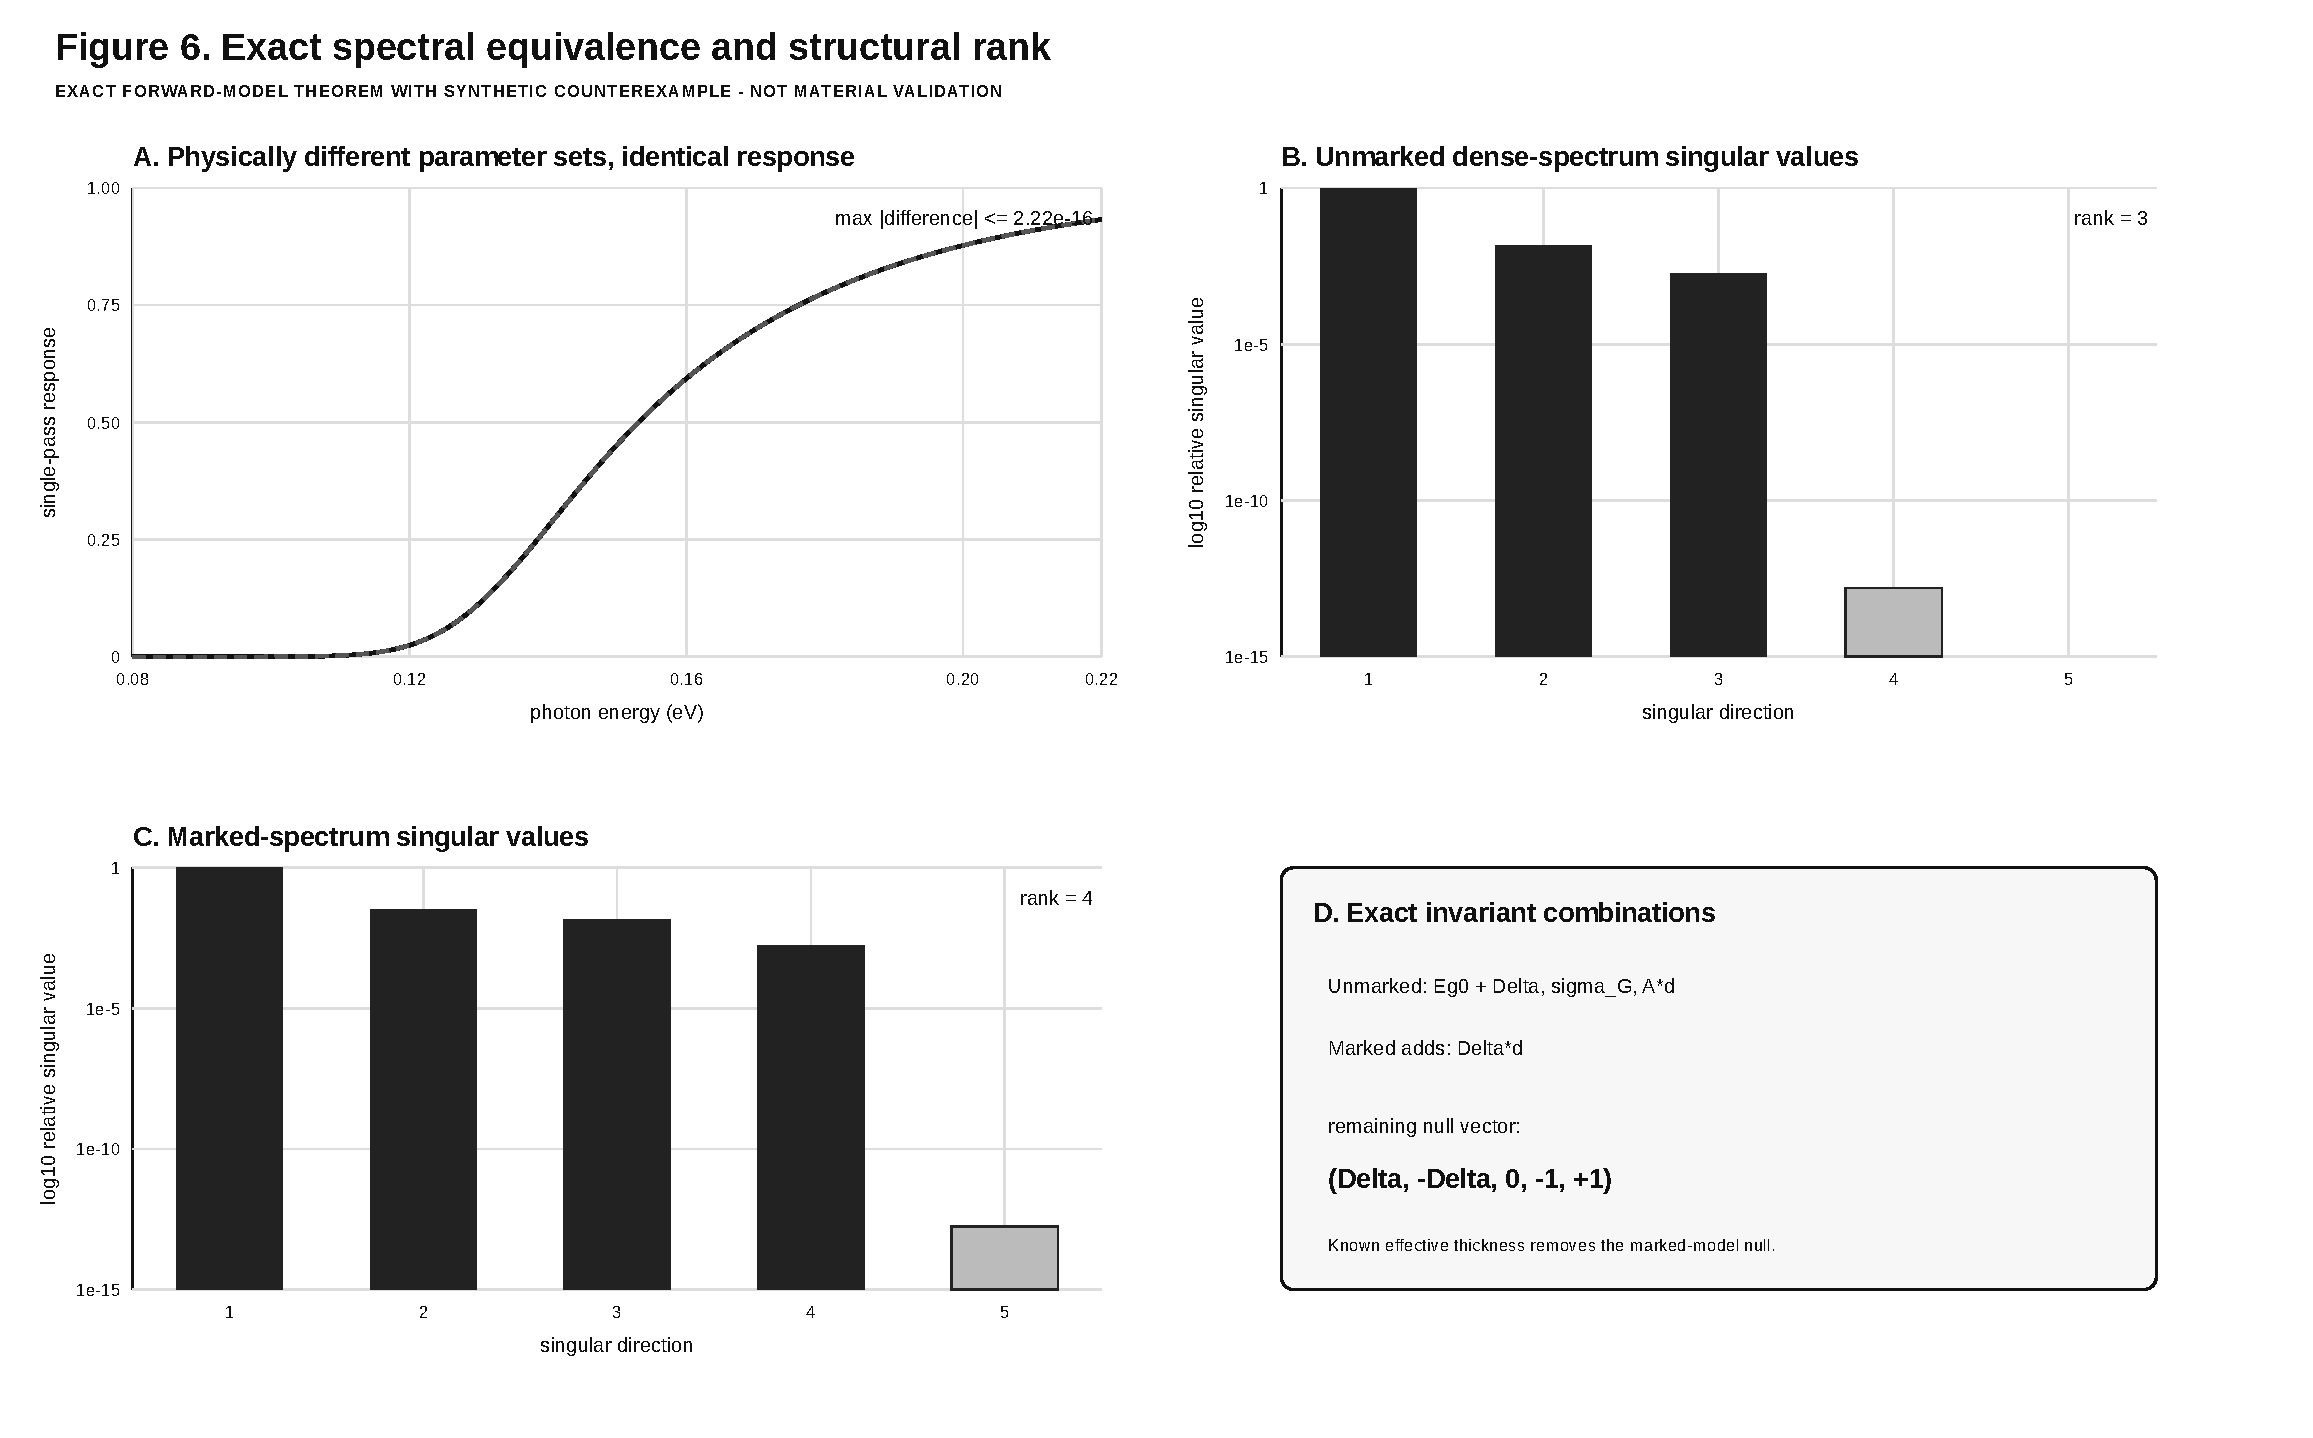
\includegraphics[width=\textwidth,height=0.82\textheight,keepaspectratio]{figures/figure6_unified_structural_rank.pdf}
\caption{Exact spectral equivalence, singular values, and structural null directions of the declared unified spectrum model.}
\label{fig:figure6:unified:structural:rank}
\end{figure}
\clearpage

For

\[
G\sim\mathcal N(E_g^{(0)}+\Delta_c,\sigma_G^2)
\]

and

\[
R(E)=1-\exp\left\{
-Ad\,\sigma_G^p
F_p\left[
\frac{E-E_g^{(0)}-\Delta_c}{\sigma_G}
\right]
\right\},
\]

the five nominal parameters

\[
(E_g^{(0)},\Delta_c,\ln\sigma_G,\ln A,\ln d)
\]

enter only through

\[
E_g^{(0)}+\Delta_c,
\qquad
\sigma_G,
\qquad
Ad.
\]

The gap-carrier combination is model-specific. The amplitude-thickness product is inherited from standard optical depth. Therefore

\[
\frac{\partial R}{\partial E_g^{(0)}}
=
\frac{\partial R}{\partial\Delta_c},
\]

\[
\frac{\partial R}{\partial\ln A}
=
\frac{\partial R}{\partial\ln d},
\]

and

\[
\boxed{\operatorname{rank}(J)\le3}.
\]

We present this as an application-specific structural-identifiability bound for the declared HgCdTe operator, not as new general identifiability mathematics.

The parameter sets

\begin{verbatim}
Eg0=0.100 eV, Delta=0.030 eV, sigma=0.010 eV, A=30000, d=10 um
Eg0=0.120 eV, Delta=0.010 eV, sigma=0.010 eV, A=15000, d=20 um
\end{verbatim}

preserve the three combinations. Across 281 spectral points, their maximum absolute response difference is

\[
2.22\times10^{-16}.
\]

The numerical singular values are

\begin{verbatim}
2.10943527e2
3.12774161e0
3.79499126e-1
3.36022167e-11
4.59184616e-14
\end{verbatim}

and the numerical rank is three.

Known carrier shift alone leaves the amplitude-thickness null direction. Known effective thickness alone leaves the gap-carrier null direction. Under the declared base model, both external constraints are required to recover the remaining latent-gap parameters separately.

\subsection{A controlled carrier marker adds one direction but leaves one scale}

Add the diagnostic carrier-sensitive term

\[
\alpha_m(E)=B\Delta_c(E_r/E)^2.
\]

The marked model depends on four combinations:

\[
E_g^{(0)}+\Delta_c,
\qquad
\sigma_G,
\qquad
Ad,
\qquad
\Delta_cd.
\]

One combined transformation remains:

\[
d\rightarrow cd,
\qquad
A\rightarrow A/c,
\qquad
\Delta_c\rightarrow\Delta_c/c,
\]

\[
E_g^{(0)}
\rightarrow
E_g^{(0)}+\Delta_c(1-1/c).
\]

The infinitesimal null vector in coordinates $(E_g^{(0)},\Delta_c,\ln\sigma_G,\ln A,\ln d)$ is

\[
(\Delta_c,-\Delta_c,0,-1,1).
\]

The marked-spectrum rank is four in the declared design. Independently known effective thickness removes the final null direction. This marker is not the Dingrong free-carrier absorption law.

\section{Discussion}

\subsection{Structural and statistical uncertainty are different}

Noise reduction and denser sampling improve estimates only inside identifiable parameter combinations. They cannot remove an exact output-preserving transformation. This is established inverse-problem logic; its consequence here is concrete. Even a continuum, noise-free spectrum cannot separate $E_g^{(0)}$ from a rigid carrier translation or absorption amplitude from effective thickness under the base model.

\subsection{A reported edge is a specimen-and-operator quantity}

A reported edge can move without a change in the latent mean gap because:

\begin{enumerate}
\item composition distributions alter local-gap and transition statistics;
\item the fitted interval changes an apparent tail energy;
\item effective thickness and response criterion move detector cutoff;
\item carrier filling and many-body terms move the interband threshold.
\end{enumerate}

A scalar edge coordinate is incomplete unless the specimen state and observation operator are declared.

\subsection{Minimum independent information}
\begin{figure}[p]
\centering
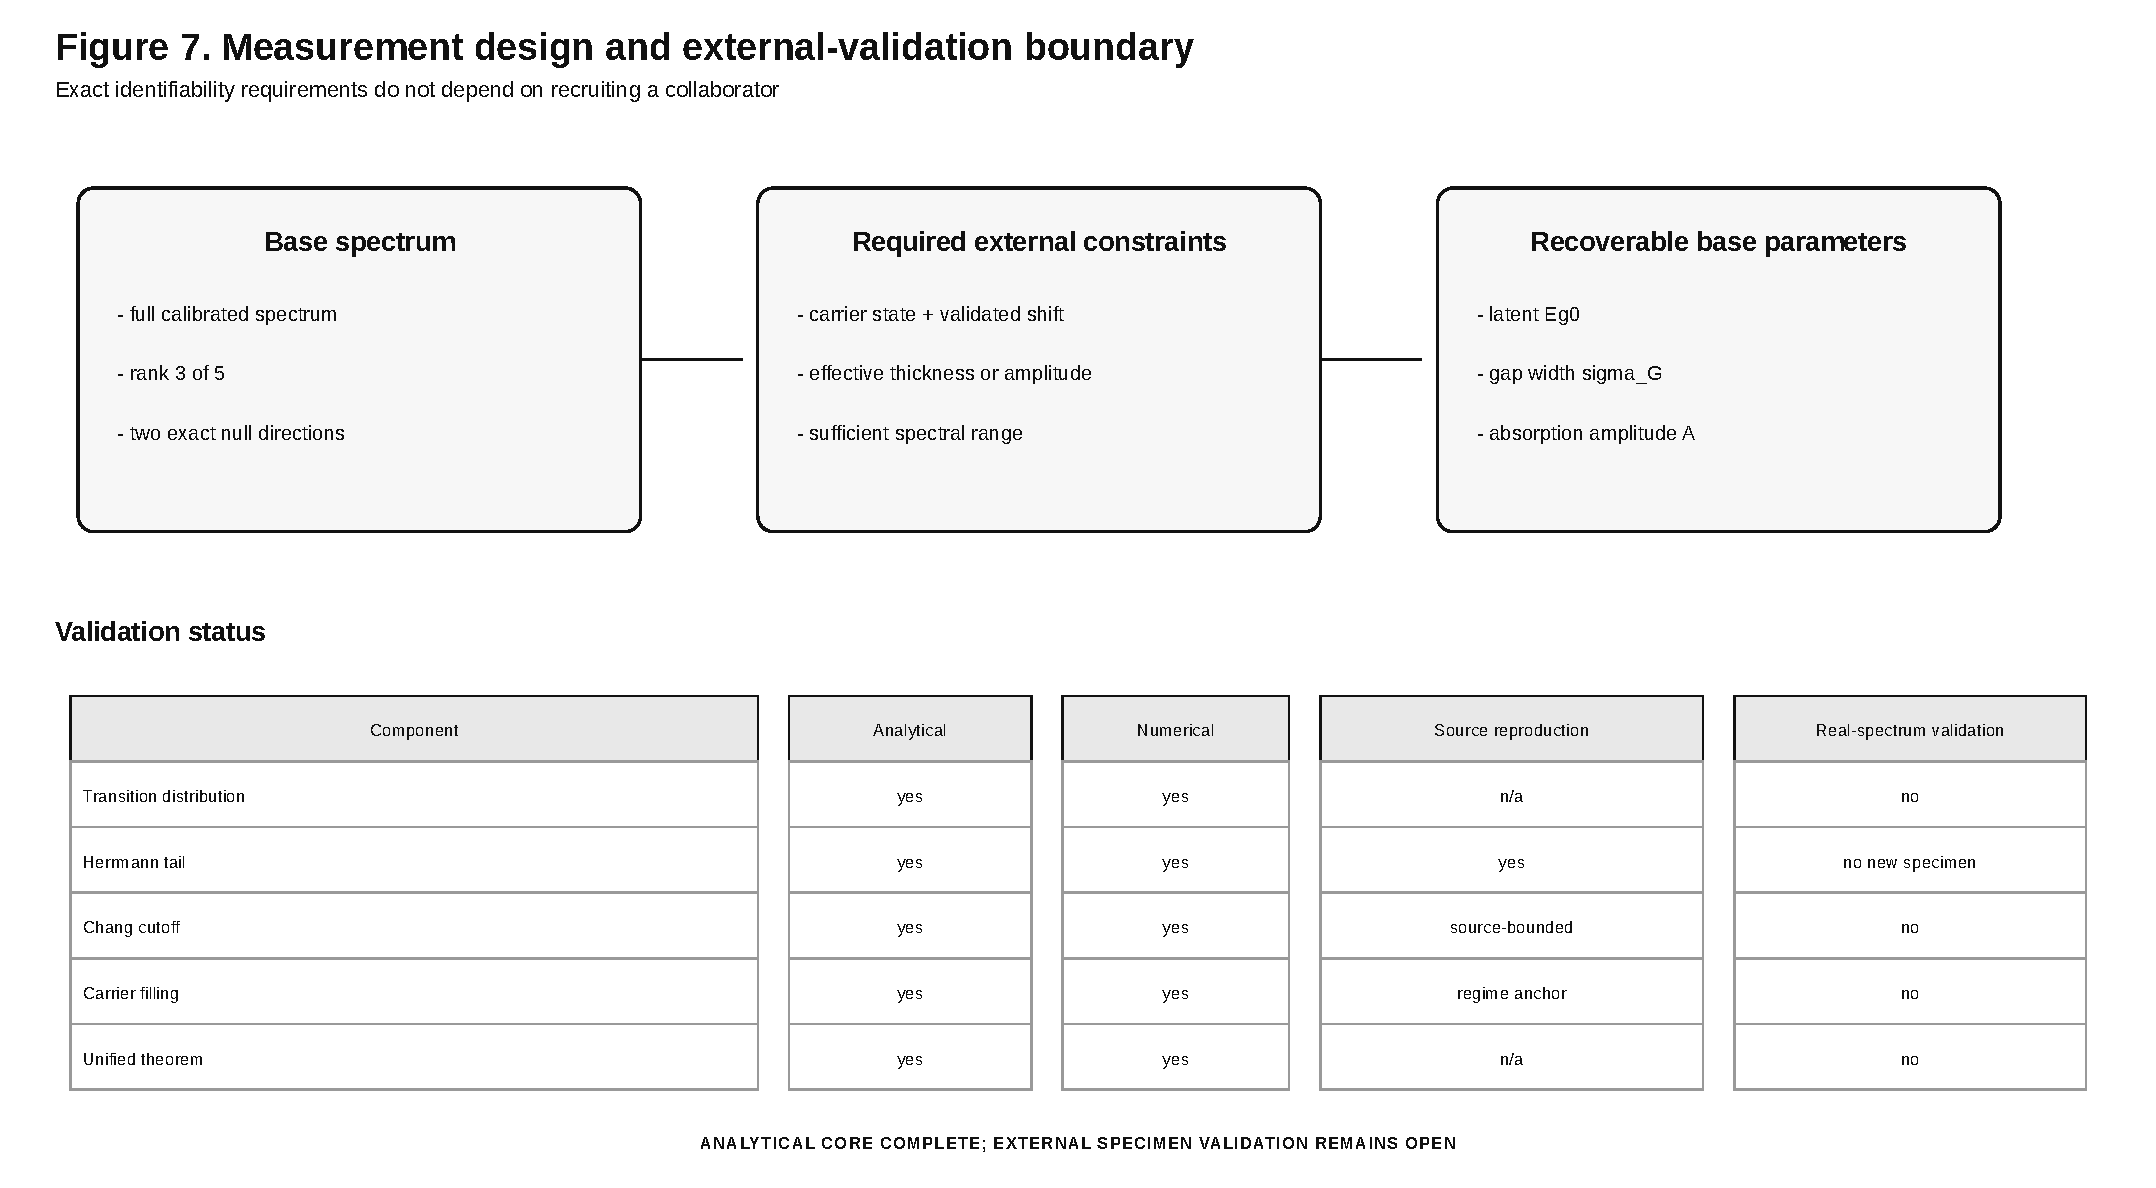
\includegraphics[width=\textwidth,height=0.82\textheight,keepaspectratio]{figures/figure7_measurement_design.pdf}
\caption{Independent information required to remove the model-specific null directions and the present external-validation boundary.}
\label{fig:figure7:measurement:design}
\end{figure}
\clearpage

Under the base model, latent-gap recovery requires at least:

\begin{itemize}
\item independent carrier-state information and a validated carrier-shift model;
\item independently calibrated effective thickness or absorption amplitude;
\item a calibrated spectrum with enough range to resolve the remaining shape parameters.
\end{itemize}

A carrier-sensitive background can add an independent direction only when its spectral form and absolute scale are retained. Removing it as an untracked baseline may discard information needed to distinguish carrier state from latent gap.

\subsection{Relation to prior work}

General structural-identifiability theory establishes the distinction between parameter fit and unique parameter recovery. Symmetry and identifiable-combination methods establish how output-preserving transformations expose unresolved directions. Beer-Lambert theory establishes the optical-depth product, while thin-film optical inversion literature demonstrates how additional observables and constraints can restore thickness and optical-constant recovery.

Herrmann et al. establish the Gaussian-gap tail mechanism. The present source-conditioned calculation reproduces the source scale and quantifies fit-window non-uniqueness.

Chang et al. establish nonparabolic-Urbach absorption and effective-thickness-dependent detector cutoff. The present work derives the application-specific tail-only rank bound and mixed-branch conditioning result. It does not present Chang's calculated thickness curve as independent validation.

Dingrong et al. establish finite-temperature carrier filling and free-carrier absorption in a real degenerate specimen. The present work reproduces the source table, exposes the printed-parameter inconsistency, and keeps the full below-gap spectrum outside the supported claim.

The contribution is the HgCdTe-specific analytical synthesis and measurement design: one forward hierarchy, explicit identifiable combinations, exact model-specific counterexamples, and quantitative evidence boundaries. Broader HgCdTe spectroscopy context includes intrinsic-absorption analysis across composition and temperature and photoluminescence studies of processing-dependent alloy disorder. \cite{chu_mi_tang_1991,ivanov_omskii_2009}

\subsection{Publication positioning}

The appropriate positioning is semiconductor optical metrology and inverse-problem methods. The exact statements may be labeled theorems because they are proved under declared assumptions, but the paper does not claim to introduce structural-identifiability mathematics. The strongest candidate contributions are:

\begin{itemize}
\item the explicit HgCdTe parameter combinations and rank bounds;
\item the machine-precision spectral counterexample;
\item the fit-window and mixed-branch quantitative results;
\item the Dingrong source-consistency audit;
\item the external-measurement prescription implied by the forward symmetries.
\end{itemize}

\section{Limitations}

\begin{enumerate}
\item Gaussian local-gap distributions may not represent clustering, gradients, or correlated disorder.
\item The power-law local edge is a sensitivity basis, not a complete Kane absorption model.
\item Carrier translation is spatially uniform in the unified theorem.
\item The generic carrier marker is not a physical free-carrier absorption model.
\item Single-pass response excludes reflection, interference, multiple paths, transport, and energy-dependent collection efficiency.
\item The zero-temperature carrier calculation is a synthetic sensitivity result; the Dingrong finite-temperature source-table reproduction is separate.
\item Dingrong native calibrated spectra, covariance, and complete Haga-Tang functions remain unavailable.
\item Chang's published thickness curve is calculated rather than an independent measured multi-thickness validation series.
\item Local opposite-sign fractions are not bulk topological invariants.
\item Structural rank does not determine practical posterior uncertainty after external constraints are supplied.
\item The prior-art audit is targeted and can be revised if a closer spectroscopy-specific source is found.
\item Complete specimen-spectrum validation remains stronger evidence than the available four-row source-table reproduction.
\end{enumerate}

\section{Conclusions}

We developed a source-grounded forward framework for HgCdTe band-edge observations and derived model-specific identifiability limits. Composition variation near inversion produces root distributions that can be censored and asymmetric. Gaussian gap distributions produce exponential-looking tails whose fitted scale changes by 60.1\% with the observation window. Effective thickness moves detector cutoff, while tail-only cutoff datasets identify at most two combinations in the declared Chang operator. Nonparabolic carrier treatment is essential in the declared high-density sensitivity case. Dingrong Table 1 provides a qualified real-specimen source test and exposes an 11.297 meV RMS inconsistency between the printed finite-temperature equation, printed momentum matrix, and reported Fermi elevations.

For the declared distributed single-state spectrum, five nominal parameters enter through only three combinations: translated mean gap, gap width, and optical-depth scale. The corresponding Jacobian rank is at most three. A controlled carrier-sensitive marker raises rank to four but leaves one combined invariance until an external scale is supplied.

The central result is methodological and material-specific:

\begin{quote}\itshape
The precision of an extracted edge is not the precision of a latent bandgap. Recovering a latent HgCdTe gap requires a forward observation model and independent constraints on the exact parameter combinations that the measurement cannot separate.
\end{quote}

\section{Reproducibility and data availability}

Quantitative results are controlled by:

\begin{itemize}
\item \texttt{data/validation/near\_critical\_transition\_model\_dependence.json};
\item \texttt{data/validation/herrmann\_gaussian\_tail\_reproduction.json};
\item \texttt{data/validation/chang\_2006\_cutoff\_identifiability.json};
\item \texttt{data/validation/dingrong\_1985\_carrier\_filling\_sensitivity.json};
\item \texttt{data/validation/dingrong1985\_table1\_reproduction.json};
\item \texttt{data/validation/unified\_spectrum\_structural\_rank.json};
\item \texttt{data/validation/flagship\_novelty\_claim\_matrix.json}.
\end{itemize}

Executable implementations are in:

\begin{itemize}
\item \texttt{src/mct\_research/distributional\_gap.py};
\item \texttt{src/mct\_research/distributional\_quadrature.py};
\item \texttt{src/mct\_research/spectral\_convolution.py};
\item \texttt{src/mct\_research/detector\_cutoff.py};
\item \texttt{src/mct\_research/carrier\_filling.py};
\item \texttt{src/mct\_research/dingrong1985.py};
\item \texttt{src/mct\_research/unified\_spectrum.py}.
\end{itemize}

The analytical derivations are in \texttt{docs/derivations/008} through \texttt{014}. Restricted source PDFs are not redistributed by the public repository.

\section{Submission status}

The analytical manuscript, deterministic figures, source-table reproduction, and audited novelty boundary are complete enough for methods-paper preparation. Remaining gates are:

\begin{enumerate}
\item complete bibliography and citation verification;
\item a journal-specific decision on whether the qualified Dingrong source-table test is sufficient or a digitized calibrated spectrum is required;
\item conversion of approved vector figures to the selected journal format;
\item author, affiliation, CRediT, funding, conflict, data/code, and archive metadata;
\item final independent review of the exact claim wording.
\end{enumerate}

A complete native-spectrum validation would strengthen the paper but is no longer represented as already available.


\appendix

\section{Controlled theorem, result, and provenance tables}

\begingroup
\scriptsize
\begin{longtable}{@{}p{0.120\linewidth}p{0.250\linewidth}p{0.240\linewidth}p{0.330\linewidth}@{}}
\caption{Exact statements and evidence classes}\\
\toprule
\textbf{Label} & \textbf{Assumptions} & \textbf{Result} & \textbf{Evidence class} \\
\midrule
\endfirsthead
\toprule
\textbf{Label} & \textbf{Assumptions} & \textbf{Result} & \textbf{Evidence class} \\
\midrule
\endhead
Proposition 1 & narrow composition distribution & mean curvature bias and local gap width & exact asymptotic \\
Proposition 2 & simple transition root & dTc/dx = -Eg\_x/Eg\_T & exact local \\
Proposition 3 & Gaussian gaps; power-law local edge & A sigma\_G\textasciicircum{}p F\_p((E-mu)/sigma\_G) & exact scale form \\
Theorem 1 & single-pass exponential tail & cutoff shift = -W ln(d2/d1) & exact \\
Theorem 2 & tail-only Chang cutoffs & rank(J\_tail) <= 2 & exact structural \\
Proposition 4 & Kane-type isotropic dispersion & exact nonparabolic positive root & exact \\
Proposition 5 & one scalar edge & rank <= 1 & exact dimensional \\
Theorem 3 & unmarked unified spectrum & rank(J) <= 3 & exact structural \\
Theorem 4 & absolutely calibrated carrier marker & rank <= 4 with combined null & exact structural \\
Corollary & base unified model & carrier and optical-scale constraints required & measurement design \\
\bottomrule
\end{longtable}
\endgroup

\begingroup
\scriptsize
\begin{longtable}{@{}p{0.220\linewidth}p{0.280\linewidth}p{0.440\linewidth}@{}}
\caption{Controlled quantitative headline results}\\
\toprule
\textbf{Result} & \textbf{Value} & \textbf{Claim state} \\
\midrule
\endfirsthead
\toprule
\textbf{Result} & \textbf{Value} & \textbf{Claim state} \\
\midrule
\endhead
Latent-law central Tc span & 25.0803 K & bounded model comparison \\
Herrmann source-window W\_fit/s & 0.50504 & source reproduction \\
Tail-energy fit-window increase & 60.1\% & synthetic observation sensitivity \\
5-to-20 um cutoff energy shift & -16.636 meV & synthetic Chang sensitivity \\
Parabolic carrier overestimate & 147.323 meV & synthetic Dingrong-regime sensitivity \\
Carrier density-series condition & 11034.75 & numerical identifiability \\
Unmarked unified rank & 3 of 5 & exact theorem + numerical verification \\
Exact-counterexample max difference & 2.22e-16 & numerical verification \\
Marked unified rank & 4 of 5 & exact theorem + numerical verification \\
\bottomrule
\end{longtable}
\endgroup

\begingroup
\scriptsize
\begin{longtable}{@{}p{0.220\linewidth}p{0.280\linewidth}p{0.440\linewidth}@{}}
\caption{Claim provenance and validation status}\\
\toprule
\textbf{Claim ID} & \textbf{Claim class} & \textbf{Current status} \\
\midrule
\endfirsthead
\toprule
\textbf{Claim ID} & \textbf{Claim class} & \textbf{Current status} \\
\midrule
\endhead
C01 & Exact asymptotic proposition & Complete \\
C02 & Eg\_x/Eg\_T & Exact local proposition plus exact bounded quadrature \\
C03 & Numerical comparison of declared latent laws & Complete \\
C04 & Bounded synthetic sensitivity & Complete \\
C05 & Source equation audit & Complete \\
C06 & Source-conditioned reproduction & Complete \\
C07 & Numerical observation-operator result & Complete \\
C08 & Bounded inverse-sensitivity result & Complete \\
C09 & Exact forward-model theorem; underlying Beer-Lambert and thickness physics are prior art & Complete \\
C10 & Bounded synthetic sensitivity & Complete \\
C11 & Exact application-specific structural theorem & Complete \\
C12 & Numerical identifiability result & Complete \\
C13 & Exact proposition & Complete \\
C14 & Bounded synthetic sensitivity & Complete \\
C15 & Numerical identifiability result & Complete \\
C16 & Exact application-specific structural theorem & Complete \\
C17 & Exact application-specific theorem plus numerical verification & Complete \\
C18 & Exact-invariance counterexample plus numerical verification & Complete \\
C19 & Exact marked-model invariance plus numerical verification & Complete \\
C20 & Corollary of exact theorem & Complete \\
C21 & External material validation & \textbf{Partial / submission blocker} \\
C22 & External/model validation & \textbf{Open} \\
C23 & External/model validation & \textbf{Partial} \\
\bottomrule
\end{longtable}
\endgroup

\section*{Author contributions}
Conceptualization; Methodology; Software; Validation; Formal analysis; Investigation; Data curation; Visualization; Writing - original draft; Writing - review and editing; Project administration.
\section*{Funding}
Funding statement requires final author confirmation before submission.
\section*{Conflict of interest}
The author declares a commercial interest in infrared photodetector modeling and consulting through Brooks Photonics.
\section*{Data availability}
The repository-generated data that support the findings of this study, together with the analysis code, immutable validation records, tests, and deterministic figure-generation scripts, will be openly available in a DOI-issuing archive. The persistent identifier will be inserted before final submission. Restricted publisher PDFs are not redistributed; source-conditioned quantities are identified by DOI and accompanied by provenance and transformation records.
\section*{Code availability}
The complete analysis implementation, tests, immutable numerical records, and deterministic figure-generation scripts will be deposited in the same DOI-issuing archive.

\begin{thebibliography}{99}
\bibitem{bellman_astrom_1970} R. Bellman and K. J. Åström 1970 On structural identifiability \textit{Mathematical Biosciences} \textbf{7} 329-339 \href{https://doi.org/10.1016/0025-5564(70)90132-X}{doi:10.1016/0025-5564(70)90132-X}.
\bibitem{yates_evans_chappell_2009} J. W. T. Yates, N. D. Evans and M. J. Chappell 2009 Structural identifiability analysis via symmetries of differential equations \textit{Automatica} \textbf{45} 2585-2591 \href{https://doi.org/10.1016/j.automatica.2009.07.009}{doi:10.1016/j.automatica.2009.07.009}.
\bibitem{eisenberg_hayashi_2014} M. C. Eisenberg and M. A. L. Hayashi 2014 Determining identifiable parameter combinations using subset profiling \textit{Mathematical Biosciences} \textbf{256} 116-126 \href{https://doi.org/10.1016/j.mbs.2014.08.008}{doi:10.1016/j.mbs.2014.08.008}.
\bibitem{iupac_beer_lambert_2025} International Union of Pure and Applied Chemistry 2025 Beer-Lambert law \textit{Compendium of Chemical Terminology (the Gold Book), 5th ed., online version 5.0.0} \href{https://doi.org/10.1351/goldbook.B00626}{doi:10.1351/goldbook.B00626}.
\bibitem{chambouleyron_1997} I. Chambouleyron, J. M. Martínez, A. C. Moretti and M. Mulato 1997 Retrieval of optical constants and thickness of thin films from transmission spectra \textit{Applied Optics} \textbf{36} 8238-8247 \href{https://doi.org/10.1364/AO.36.008238}{doi:10.1364/AO.36.008238}.
\bibitem{babeva_kitova_konstantinov_2001_error} T. Babeva, S. Kitova and I. Konstantinov 2001 Photometric methods for determining the optical constants and the thicknesses of thin absorbing films: selection of a combination of photometric quantities on the basis of error analysis \textit{Applied Optics} \textbf{40} 2675-2681 \href{https://doi.org/10.1364/AO.40.002675}{doi:10.1364/AO.40.002675}.
\bibitem{babeva_kitova_konstantinov_2001_unique} T. Babeva, S. Kitova and I. Konstantinov 2001 Photometric methods for determining the optical constants and the thicknesses of thin absorbing films: criteria for precise and unambiguous determination of n, k, and d in a wide spectral range \textit{Applied Optics} \textbf{40} 2682-2686 \href{https://doi.org/10.1364/AO.40.002682}{doi:10.1364/AO.40.002682}.
\bibitem{mendoza_galvan_2021} A. Mendoza-Galván, J. G. Méndez-Lara, R. A. Mauricio-Sánchez, K. Järrendahl and H. Arwin 2021 Effective absorption coefficient and effective thickness in attenuated total reflection spectroscopy \textit{Optics Letters} \textbf{46} 872-875 \href{https://doi.org/10.1364/OL.418277}{doi:10.1364/OL.418277}.
\bibitem{herrmann_1992} K. H. Herrmann, K.-P. Möllmann and J. W. Tomm 1992 Broadening mechanisms near the E0 transition in narrow-gap Hg1-xCdxTe (0.2 < x < 0.6) \textit{Journal of Crystal Growth} \textbf{117} 758-762 \href{https://doi.org/10.1016/0022-0248(92)90851-9}{doi:10.1016/0022-0248(92)90851-9}.
\bibitem{chang_2006} Y. Chang, C. H. Grein, S. Sivananthan, M. E. Flatté, V. Nathan and S. Guha 2006 Narrow gap HgCdTe absorption behavior near the band edge including nonparabolicity and the Urbach tail \textit{Applied Physics Letters} \textbf{89} 062109 \href{https://doi.org/10.1063/1.2245220}{doi:10.1063/1.2245220}.
\bibitem{chang_2007} Y. Chang, S. Guha, C. H. Grein, S. Velicu, M. E. Flatté, V. Nathan and S. Sivananthan 2007 Absorption of narrow-gap HgCdTe near the band edge including nonparabolicity and the Urbach tail \textit{Journal of Electronic Materials} \textbf{36} 1000-1006 \href{https://doi.org/10.1007/s11664-007-0162-0}{doi:10.1007/s11664-007-0162-0}.
\bibitem{dingrong_1985} Q. Dingrong, T. Wenguo, S. Jie, C. Junhao and Z. Guozhen 1985 Infrared absorption in In-doped degenerate Hg1-xCdxTe \textit{Solid State Communications} \textbf{56} 813-816 \href{https://doi.org/10.1016/0038-1098(85)90315-1}{doi:10.1016/0038-1098(85)90315-1}.
\bibitem{teppe_2016} F. Teppe, M. Marcinkiewicz, S. S. Krishtopenko, S. Ruffenach, C. Consejo, A. M. Kadykov, W. Desrat, D. But, W. Knap, J. Ludwig, S. Moon, D. Smirnov, M. Orlita, Z. Jiang, S. V. Morozov, V. I. Gavrilenko, N. N. Mikhailov and S. A. Dvoretskii 2016 Temperature-driven massless Kane fermions in HgCdTe crystals \textit{Nature Communications} \textbf{7} 12576 \href{https://doi.org/10.1038/ncomms12576}{doi:10.1038/ncomms12576}.
\bibitem{ivanov_omskii_2009} V. I. Ivanov-Omskii, N. L. Bazhenov, K. D. Mynbaev, V. A. Smirnov, V. S. Varavin, N. N. Mikhailov and G. Yu. Sidorov 2009 Study of alloy disorder in (Hg,Cd)Te with the use of infrared photoluminescence \textit{Physica B: Condensed Matter} \textbf{404} 5035-5037 \href{https://doi.org/10.1016/j.physb.2009.08.210}{doi:10.1016/j.physb.2009.08.210}.
\bibitem{chu_mi_tang_1991} J. H. Chu, Z. Y. Mi and D. Y. Tang 1991 Intrinsic absorption spectroscopy and related physical quantities of narrow-gap semiconductors Hg1-xCdxTe \textit{Infrared Physics} \textbf{32} 195-211 \href{https://doi.org/10.1016/0020-0891(91)90110-2}{doi:10.1016/0020-0891(91)90110-2}.
\end{thebibliography}


\end{document}